\documentclass[letterpaper,10pt]{article}
\usepackage[letterpaper, hmargin=1.8cm, vmargin = 2.5cm]{geometry} %Sets the page geometry
\usepackage{url}
\usepackage{hyperref}
\usepackage{multicol}
\usepackage[english]{babel}
\usepackage{setspace}
\setlength{\parskip}{1em} % Set space when paragraphs are used
\setlength{\parindent}{0in}

\usepackage{xcolor}
\usepackage{multicol}
\usepackage{float}
\usepackage{graphicx} % Package for \includegraphics
\usepackage{wrapfig} % Figure wrapping
\usepackage[T1]{fontenc} % Output font encoding for international characters
\usepackage{amssymb}
\usepackage{amsmath}
\numberwithin{equation}{section}

\usepackage{amsthm}
\usepackage{mathtools}
\usepackage{thmtools}
\usepackage{bbm}
\usepackage[autostyle]{csquotes}
\usepackage{doi}
\usepackage[
    backend=biber,
    style=authoryear-comp,
    natbib=true,
    sortlocale=en_US,
    url=false, 
    doi=true,
    eprint=false
]{biblatex}

\addbibresource{bibliography.bib}

% Other
\newtheorem{thm}{Theorem}
\numberwithin{thm}{section}
\newtheorem{dfn}{Definition}
\newtheorem{lem}{Lemma}
\numberwithin{lem}{section}
\newtheorem{rmk}{Remark}
\newtheorem{cor}{Corollary}
\numberwithin{cor}{section}
% \newtheorem{prop}{Proposition}
\newtheorem{asm}{Assumption}

\renewcommand\qedsymbol{$\blacksquare$}

\newcommand{\sumi}{\sum_{i=1}^n}
\newcommand{\calE}{\mathcal{E}}
\makeatother
\renewcommand{\hat}{\widehat}
\newcommand{\E}{\mathbb{E}}
\newcommand{\1}{\mathbbm{1}}
\newcommand{\Var}{\text{Var}}
\newcommand{\Cov}{\text{Cov}}
\newcommand{\rk}{\text{rk}}
\renewcommand{\P}{\mathbbm{P}}

\makeatletter
\def\blfootnote{\gdef\@thefnmark{}\@footnotetext}
\makeatother

\DeclarePairedDelimiter\floor{\lfloor}{\rfloor} %Floor function
\DeclarePairedDelimiter\ceil{\lceil}{\rceil} %Ceil function
\DeclareMathOperator*{\argmax}{arg\,max} % argmax
\DeclareMathOperator*{\argmin}{arg\,min} % argmin
\newcommand{\indep}{\perp\!\!\!\!\perp} 


\begin{document}
\singlespacing
\title{Pointwise and Uniform Inference for the Two-Scale\\ Distributional Nearest Neighbor Estimator}
\date{Last edited: \today}
\author{Jakob R. Juergens \\ University of Wisconsin - Madison}
\maketitle
\hrule
\onehalfspacing
\begin{abstract}
	Recent advances in the literature on non-parametric regression and uniform inference for infinite-order U-statistics have enabled us to consider the problem of uniform inference for a broader class of estimators.
	One class of such estimators are bagged nearest neighbor estimators and among them specifically the Two-Scale Distributional Nearest Neighbor Estimator (TDNN) of \citet{demirkaya_optimal_2024}.
	In this paper, we improve on existing results for pointwise inference using the TDNN estimator and develop uniform inference procedures based on recent work by \citet{ritzwoller_uniform_2024}.
	As part of this work, we provide a complementary R package called \textit{tdnnR} that implements the presented methods.

	% \blfootnote{The author thanks Harold D. Chiang, Jack Porter {\color{red} ADD OTHERS} for invaluable feedback.}
\end{abstract}
\vspace{0.3cm}
\hrule
\singlespacing

\vspace{-0.3cm}
\begin{center}
	{\small Supplementary Material and R Package available at: \url{https://github.com/JakobJuergens/Unif_Inf_TDNN}}
\end{center}
\vspace{0.3cm}
\hrule
\singlespacing
% {\small \tableofcontents}
\thispagestyle{empty}

\pagenumbering{arabic}

\newpage
\onehalfspacing
\section{Introduction}
\hrule
Nearest Neighbor Estimators and their derivatives form a flexible class of estimators for a variety of purposes including nonparametric regression.
Although widely used in practice for the latter purpose, some of their properties are still elusive when it comes to performing inference.
	{\color{red} LOREM IPSUM}
Due to the inherent connection of the Potential Nearest Neighbors (PNN) framework to Random Forests (RF), this work also contributes to contextualizing recent advances in inference techniques for random forests.
	{\color{red} LOREM IPSUM}

The remainder of this paper is organized as follows.
Section \ref{sec:TDNN} introduces the TDNN estimator as developed by \citet{demirkaya_optimal_2024} and presents some of the results this paper is based on.
Section \ref{sec:pw_inf} uses recent theoretical developments to show that the distributional approximations provided by \citet{demirkaya_optimal_2024} can be justified under weaker assumptions on the chosen subsampling scales.
Section \ref{unif_inf} extends results from \citet{ritzwoller_uniform_2024} to the TDNN estimator and thus introduces methods to construct uniform confidence bands for the TDNN estimator.
Section \ref{Simulations} explores the performance of the developed uniform inference methods in a number of setups and Section \ref{Application} applies them to the context of {\color{red} LOREM IPSUM}.
Section \ref{Conclusion} concludes.

\subsection{Notation}
In the following, $\rightsquigarrow$ denotes convergence in distribution.
The norm $\| \cdot \|_{\psi_1}$ denotes the $\psi_1$-Orlicz norm.
Recall that random variables are sub-exponential if and only if they have a finite $\psi_1$-Orlicz norm.
Let $[n] = \{1, \dotsc, n\}$.
To simplify notation going forward, we introduce two sets that will be used extensively.
\begin{equation}
	L_{n,s} = \left\{\left(l_1, \dotsc, l_s\right) \in [n]^{s} \, : \, \text{entries of vector are distinct} \right\}
	\quad \text{and} \quad
	I_{n,s} = \left\{\left(i_1, \dotsc, i_s\right) \in L_{n,s} \, : \, i_1 < \dotsc < i_s \right\}
\end{equation}
Similarly, given a finite index set $\mathcal{I} \subset \mathbb{N}$, define the following sets.
\begin{equation}
	L_{s}(\mathcal{I}) = \left\{\left(l_1, \dotsc, l_s\right) \in \mathcal{I}^{s} \, : \, \text{entries of vector are distinct} \right\}
	\quad \text{and} \quad
	I_{s}(\mathcal{I}) = \left\{\left(i_1, \dotsc, i_s\right) \in L_{s}(\mathcal{I}) \, : \, i_1 < \dotsc < i_s \right\}
\end{equation}
{\color{red} TO-DO:}
\begin{itemize}
	\item $\lesssim$ needs an explanation
\end{itemize}


\newpage
\section{Two-Scale Distributional Nearest Neighbor Estimator}\label{sec:TDNN}
\hrule
As in \citet{demirkaya_optimal_2024}, consider a sample of independent and identically distributed observations
\begin{equation}\label{DGP}
	\mathbf{D}_n = \{\mathbf{Z}_i = (\mathbf{X}_i, Y_i)\}_{i = 1}^{n}
	\quad \text{from the model} \quad
	Y = \mu(\mathbf{X}) + \varepsilon,
\end{equation}
where $Y \in \mathbb{R}$ is the response, $\mathbf{X} \in \mathbb{R}^d$ is a feature vector of fixed dimension $d$, and $\mu(\mathbf{x})$ is the unknown mean regression function.
$\varepsilon$ is the unobservable model error on which we impose the following conditions.
\begin{equation}
	\varepsilon \indep \mathbf{X}, \quad
	\E\left[\varepsilon\right] = 0, \quad
	\Var\left(\varepsilon\right) = \sigma_{\varepsilon}^2
\end{equation}
We will denote the distribution induced by this model by $P$ and thus $\mathbf{Z}_i \overset{\text{iid}}{\sim} P$.
As we will embed the corresponding estimation problem in the context of subsampled conditional moment regression, note that this implies a conditional moment equation of the form
\begin{equation}\label{CondMomEq}
	M(\mathbf{x}; \mu)
	= \E\left[m(\mathbf{Z}_i; \mu) \, | \, \mathbf{X}_i = \mathbf{x}\right]
	= 0
	\quad \text{where} \quad
	m(\mathbf{Z}_i; \mu) = Y_i - \mu(\mathbf{X}_i).
\end{equation}
Due to the absence of nuisance parameters in the setting at hand, conditions such as local Neyman-orthogonality vacuously hold (uniformly).
In practice, the non-parametric regression problem at hand can be approached by solving the corresponding empirical conditional moment equation.
\begin{equation}\label{EmpCondMomEq}
	M_n(\mathbf{x}; \mu, \mathbf{D}_n)
	= \sum_{i = 1}^{n}K(\mathbf{x}, \mathbf{X}_i)m(\mathbf{Z}_i; \mu)
	= 0
\end{equation}
In this equation, $K:\mathbb{R}^d \times \mathbb{R}^d \rightarrow \mathbb{R}$ is a data-dependent Kernel function measuring the ``distance'' between the point of interest and an observation.
Notationally, this makes the local and data-dependent approach of this procedure explicit.

\subsection{Distributional Nearest Neighbor Estimator}
One estimator that fulfills the purpose of estimating $\mu$ nonparametrically is the Distributional Nearest Neighbor (DNN) estimator.
With a name coined by \citet{demirkaya_optimal_2024}, the DNN estimator is based on important work by \citet{steele_exact_2009} and \citet{biau_rate_2010}.
Given a sample as described above and a fixed feature vector $\mathbf{x}$, consider the ordered sample $\{(\mathbf{X}_{(1)}, Y_{(1)}), \dotsc, (\mathbf{X}_{(n)}, Y_{(n)})\}$ defined by
\begin{equation}\label{ordering}
	||\mathbf{X}_{(1)} - \mathbf{x}|| \leq ||\mathbf{X}_{(2)} - \mathbf{x}|| \leq \dotsc \leq ||\mathbf{X}_{(n)} - \mathbf{x}||
\end{equation}
where draws are broken according to the natural indices of the observations in a deterministic way.
Let $\rk(\mathbf{x}; \mathbf{Z}_i, D)$ denote the \textit{rank} that is assigned to observation $i$ in a sample $D$ relative to a point of interest $\mathbf{x}$ in this fashion.
By convention, let $\rk(\mathbf{x}; \mathbf{Z}_i, D) = \infty$ if $\mathbf{Z}_i \not\in D$.
Similarly, let $Y_{(1)}(\mathbf{x}; D)$ indicate the response value of the closest neighbor in set $D$.
Depending on the underlying norm that is used to calculate the distances between observations, it can be advisable to standardize the feature space before applying nearest-neighbor methods.
Since this is highly context-dependent, it is impossible to give general advice on when to standardize.

Given a subsampling scale $s$ satisfying $1 \leq s \leq n$, a generic set of subsample indices $\ell \in L_{n,s}$ and a corresponding generic subset of our data $D_{\ell} = \{\mathbf{Z}_i \, | \, i \in \ell\}$, we can consider an analogous ordering of $D_{\ell}$.
This enables us to define a data-driven kernel function $\kappa$ following the notation of \citet{ritzwoller_uniform_2024}.
\begin{equation}
	\kappa(\mathbf{x}; \mathbf{Z}_i, D_{\ell}, \xi)
	= \1\left(\rk(\mathbf{x}; \mathbf{Z}_i, D_{\ell}) = 1\right)
\end{equation}
Here, $\xi$ is an additional source of randomness in the construction of the base learner that comes into play when analyzing, for example, random forests as proposed by \citet{breiman_random_2001} using the CART-algorithm described in \citet{breiman_classification_2017}.
As the DNN estimator does not incorporate such additional randomness, the term is omitted in further considerations.
Noteworthy properties of $\kappa$ are its permutational symmetry in $D_{\ell}$ and that $\kappa$ does not consider the response variable when assigning weights to the observations under consideration.
The latter immediately implies a property that has been called ``Honesty'' by \citet{wager_estimation_2018}.

\begin{dfn}[Symmetry and Honesty - Adapted from \citet{ritzwoller_uniform_2024}]\label{Symmetry_Honesty}\mbox{}
	\begin{enumerate}
		\item The kernel $\kappa\left(\cdot, \cdot, D_{\ell}\right)$ is Honest in the sense that
		      $$\kappa\left(\mathbf{x}, \mathbf{X}_i, D_{\ell}\right) \indep m\left(\mathbf{Z}_i ; \mu\right) \mid \mathbf{X}_i, D_{\ell,-i},$$
		      where $\indep$ denotes conditional independence and $D_{\ell,-i} = \{\mathbf{Z}_l \, | \, l \in \ell \backslash \{i\}\}$.
		\item The kernel $\kappa\left(\cdot, \cdot, D_{\ell}\right)$ is positive and satisfies the restriction
		      $\sum_{i \in s} \kappa\left(\cdot, \mathbf{X}_i, D_{\ell}\right)=1$ almost surely.
		      Moreover, the kernel $\kappa\left(\cdot, \mathbf{X}_i, D_{\ell}\right)$ is invariant to permutations of the data $D_{\ell}.$
	\end{enumerate}
\end{dfn}
Using $\kappa$, it is straightforward to find an expression for the distance function $K$ in Equation \ref{EmpCondMomEq} corresponding to the DNN estimator.
\begin{equation}
	K(\mathbf{x}, \mathbf{X}_i)
	= \binom{n}{s}^{-1} \sum_{\ell \in L_{n,s}} \1(i \in \ell)\frac{\kappa(\mathbf{x}; \mathbf{Z}_i, D_{\ell})}{s!}
	= \binom{n}{s}^{-1} \sum_{\ell \in L_{n,s}} \frac{\1\left(\rk(\mathbf{x}; \mathbf{Z}_i, D_{\ell}) = 1\right)}{s!}
\end{equation}
Inserting into Equation \ref{EmpCondMomEq}, this gives us the following empirical conditional moment equation.
\begin{equation}
	\begin{aligned}
		M_n(\mathbf{x}; \mu, \mathbf{D}_n)
		 & = \sum_{i = 1}^{n}K(\mathbf{x}, \mathbf{X}_i)m(\mathbf{Z}_i; \mu)                                                                                                                  \\
		 & = \sum_{i = 1}^{n}\left(\binom{n}{s}^{-1} \sum_{\ell \in L_{n,s}} \frac{\1\left(\rk(\mathbf{x}; \mathbf{Z}_i, D_{\ell}) = 1\right)}{s!}\right)\left(Y_i - \mu(\mathbf{X}_i)\right)
		= 0
	\end{aligned}
\end{equation}
Solving this empirical conditional moment equation then yields the DNN estimator $D_{n}^{s}(\mathbf{x})$ with subsampling scale $s$ estimating the conditional expectation function $\mu(\mathbf{x}) = \E\left[Y \, | \, \mathbf{X} = \mathbf{x}\right]$.
After rearranging the terms, it is given by the following U-statistic.
\begin{equation}\label{U_stat}
	\tilde{\mu}_{s}(\mathbf{x}; \mathbf{D}_n)
	%= \binom{n}{s}^{-1} \sum_{\iota \in I_{n,s}} h_{\mathbf{x}}(D_{\iota})
	= \binom{n}{s}^{-1} \sum_{\ell \in L_{n,s}} \frac{1}{s!} Y_{(1)}(\mathbf{x}; D_{\ell})
	=: \binom{n}{s}^{-1} \sum_{\ell \in L_{n,s}} h_{s}(\mathbf{x}; D_{\ell})
\end{equation}

From the empirical conditional moment equation, it becomes apparent that the DNN estimator is a Weighted Nearest Neighbor (WNN) estimator that automatically assigns suitable weights in a distributional fashion.
Weighted nearest neighbor estimators in their general form have been studied in detail by {\color{red} ADD REFERENCES}.
Among other properties, it has been shown that under smoothness assumptions and using a suitable weight vector their convergence rate is optimal with $O_p(n^{-\frac{2}{d+4}}).$
Through an equivalent representation as an L-statistic developed by \citet{steele_exact_2009}, the estimator has a computationally simple way to be evaluated compared to the usual U-statistic approach.

\subsection{Two-Scale Distributional Nearest Neighbor Esimator}
Starting from this setup, \citet{demirkaya_optimal_2024} develop a novel bias-correction method for the DNN estimator that leads to appealing finite-sample properties of the resulting Two-Scale Distributional Nearest Neighbor (TDNN) estimator.
Their method is based on an explicit formula for the first-order bias term of the DNN estimator, which in turn allows them to eliminate it through a clever combination of two DNN estimators.

\begin{thm}[\citet{demirkaya_optimal_2024} - Theorem 1]\label{thm:dem1}\mbox{}\\*
	Assume that the distribution of $\mathbf{X}$ has a density function $f(\cdot)$ with respect to the Lebesgue measure $\lambda$ on the Euclidean space $\mathbb{R}^d$.
	Let $\mathbf{x} \in \operatorname{supp}(\mathbf{X})$ be a fixed feature vector.
	If \dots
	\begin{enumerate}
		\item There exists some constant $\alpha>0$ such that $\mathbb{P}(\|\mathbf{X}-\mathbf{x}\| \geq R) \leq e^{-\alpha R}$ for each $R>0$.
		\item The density $f(\cdot)$ is bounded away from 0 and $\infty, f(\cdot)$ and $\mu(\cdot)$ are four times continuously differentiable with bounded second, third, and fourth-order partial derivatives in a neighborhood of $\mathbf{x}$, and $\E[Y^2]<\infty$.
		      Moreover, the model error $\varepsilon$ has zero mean and finite variance $\sigma_\epsilon^2>0$ and is independent of $\mathbf{X}$.
		\item We have an i.i.d. sample $\left\{\left(\mathbf{X}_1, Y_1\right),\left(\mathbf{X}_2, Y_2\right), \dotsc,\left(\mathbf{X}_n, Y_n\right)\right\}$ of size $n$ from the model described in Equation \ref{DGP}.
	\end{enumerate}
	Then, for any fixed $\mathbf{x} \in$ $\operatorname{supp}(\mathbf{X}) \subset \mathbb{R}^d$, we have that as $s \rightarrow \infty$
	\begin{equation}
		\E\left[\tilde{\mu}_{s}(\mathbf{x}; \mathbf{D}_n)\right] = \mu(\mathbf{x})+B(s)
	\end{equation}
	with
	\begin{align*}
		B(s) & =\Gamma(2 / d+1) \frac{f(\mathbf{x}) \operatorname{tr}\left(\mu^{\prime \prime}(\mathbf{x})\right)+2 \mu^{\prime}(\mathbf{x})^T f^{\prime}(\mathbf{x})}{2 d V_d^{2 / d} f(\mathbf{x})^{1+2 / d}} s^{-2 / d}+R(s) \\
		R(s) & = \begin{cases}O\left(s^{-3}\right),     & d=1      \\
             O\left(s^{-4 / d}\right), & d \geq 2\end{cases}
	\end{align*}
	where\dots
	\begin{multicols}{2}
		\begin{itemize}
			\item $V_d=\frac{d^{d / 2}}{\Gamma(1+d / 2)}$
			\item $\Gamma(\cdot)$ is the gamma function
			\item $\operatorname{tr}(\cdot)$ stands for the trace of a matrix
			\item $f^{\prime}(\cdot)$ and $\mu^{\prime}(\cdot)$ denote the first-order gradients of $f(\cdot)$ and $\mu(\cdot)$, respectively
			\item $f^{\prime \prime}(\cdot)$ and $\mu^{\prime \prime}(\cdot)$ represent the $d \times d$ Hessian matrices of $f(\cdot)$ and $\mu(\cdot)$, respectively
		\end{itemize}
	\end{multicols}
\end{thm}
Choosing two subsampling scales $1 \leq s_1 < s_2 \leq n$ and two corresponding weights
\begin{equation}
	w_1^{*}(s_1, s_2) = \frac{1}{1-(s_1/s_2)^{-2/d}}
	\quad\text{and}\quad
	w_2^{*}(s_1, s_2) = 1 - w_1^{*}(s_1, s_2)
\end{equation}
they define the corresponding TDNN estimator as follows.
\begin{equation}
	\hat{\mu}_{s_1, s_2}\left(\mathbf{x}; \mathbf{D}_n\right)
	= w_1^{*}(s_1, s_2)\tilde{\mu}_{s_1}\left(\mathbf{x}; \mathbf{D}_n\right) + w_2^{*}(s_1, s_2)\tilde{\mu}_{s_2}\left(\mathbf{x}; \mathbf{D}_n\right)
\end{equation}
As a direct consequence of Theorem \ref{thm:dem1}, this leads to the elimination of the first-order bias term leading to desirable finite-sample properties.
Furthermore, the authors show that this construction improves the quality of the normal approximation.


\begin{thm}[\citet{demirkaya_optimal_2024} - Theorem 3]\label{thm:dem3}\mbox{}\\*
	Assume that Conditions (1) to (3) from Theorem \ref{thm:dem1} hold.
	Furthermore, let $s_2 \rightarrow \infty$ with $s_2 = o(n)$ and $c_1 \leq s_1/s_2 \leq c_2$ for some constants $0 < c_1 < c_2 < 1$.
	Then, for any fixed $\mathbf{x} \in \operatorname{supp}(\mathbf{X}) \subset \mathbb{R}^d,$ it holds that for some positive sequence $\sigma_n$ of order $(s_2/n)^{1/2}$,
	\begin{equation}
		\sigma_n^{-1} \left(\hat{\mu}_{s_1, s_2}\left(\mathbf{x}; \mathbf{D}_n\right) - \mu(\mathbf{x}) - \Lambda\right) \rightsquigarrow \mathcal{N}(0,1)
	\end{equation}
	as $n \rightarrow \infty$, where
	\begin{equation*}
		\Lambda = \begin{cases}
			O\left(s_1^{-4/d} + s_2^{-4/d}\right) & \text{for } d \geq 2 \\
			O\left(s_1^{-3} + s_2^{-3}\right)     & \text{for } d = 1    \\
		\end{cases}.
	\end{equation*}
\end{thm}

\subsection{U-Statistic Representation for the DNN and TDNN Estimators}
As the majority of the theoretical results in the original paper rely on representations as a U-statistic, it is necessary to introduce additional concepts and notation.
Recalling Equation \ref{U_stat}, the DNN and TDNN estimators can be expressed in the following U-statistic form and are thus a type of generalized complete U-statistic as introduced by \citet{peng_rates_2022}.
\begin{equation}
	\tilde{\mu}_{s}(\mathbf{x}; \mathbf{D}_n)
	= \binom{n}{s}^{-1} \sum_{\ell \in L_{n,s}} h_{s}(\mathbf{x}; D_{\ell})
	\quad \text{and} \quad
	\hat{\mu}_{s_1, s_2}(\mathbf{x}; \mathbf{D}_n)
	= \binom{n}{s}^{-1} \sum_{\ell \in L_{n,s_2}} h_{s_1, s_2}(\mathbf{x}; D_{\ell})
\end{equation}
It is worth pointing out that in contrast to the DNN estimator, the kernel for the TDNN estimator is of order $s_2 > s_1$.
The authors derive an explicit formula for the kernel that shows the connection between the DNN and TDNN estimators.
This connection will prove useful going forward.
\begin{lem}[Kernel of TDNN Estimator - Adapted from Lemma 8 of \citet{demirkaya_optimal_2024}]\label{lem:dem8}\mbox{}\\*
	The kernel of the TDNN estimator takes the following form.
	\begin{equation}
		\begin{aligned}
			h_{s_1, s_2}\left(\mathbf{x}; D\right)
			 & = w_{1}^{*}\left[\binom{s_2}{s_1}^{-1}\sum_{\ell \in L_{s_2, s_1}} h_{s_1}\left(\mathbf{x}; D_{\ell}\right)\right] + w_{2}^{*} h_{s_2}\left(\mathbf{x}; D\right) \\
			 & = w_{1}^{*} \tilde{\mu}_{s_1}\left(\mathbf{x}; D\right) + w_{2}^{*} h_{s_2}\left(\mathbf{x}; D\right)                                                            \\
		\end{aligned}
	\end{equation}
\end{lem}
Borrowing the notational conventions from \citet{lee_u-statistics_2019}, additionally, introduce the following notation.
\begin{equation}\label{eq:psi_s_c}
	\psi_{s}^{c}(\mathbf{x}; \mathbf{z}_{1}, \dotsc, \mathbf{z}_{c})
	= \E_{D}\left[h_{s}\left(\mathbf{x}; D\right) \, | \,  \mathbf{Z}_1 = \mathbf{z}_{1}, \dotsc, \mathbf{Z}_c = \mathbf{z}_{c}\right]
\end{equation}
\begin{equation}
	h_{s}^{(1)}\left(\mathbf{x}; \mathbf{z}_{1}\right)
	= \psi_{s}^{1}(\mathbf{x}; \mathbf{z}_{1}) - \mu(\mathbf{x})
\end{equation}
\begin{equation}
	h_{s}^{(c)}\left(\mathbf{x}; \mathbf{z}_{1}, \dotsc, \mathbf{z}_{c}\right)
	= \psi_{s}^{c}(\mathbf{x}; \mathbf{z}_{1}, \dotsc, \mathbf{z}_{c}) - \sum_{j = 1}^{c-1}\left(\sum_{\ell \in L_{n,j}}h_{s}^{(j)}(\mathbf{x}; \mathbf{z}_{\ell})\right) - \mu(\mathbf{x})
	\quad \text{for } c = 2, \dotsc, s
\end{equation}
In contrast to the notational inspiration, the subsampling size $s$ is made explicit.
Since we are dealing with an infinite-order U-statistic, $s$ will be diverging with $n$.
Completely analogous, define the corresponding objects for the TDNN estimator.
For the DNN estimator and any $1 \leq c \leq s$, define
\begin{equation}\label{eq:xi_s_c}
	\xi_{s}^{c}\left(\mathbf{x}\right)
	= \Var_{1:c}\left(\psi_{s}^{c}(\mathbf{x}; \mathbf{Z}_{1}, \dotsc, \mathbf{Z}_{c})\right)
\end{equation}
where $\mathbf{Z}_{c+1}^{\prime}, \ldots, \mathbf{Z}_n^{\prime}$ are i.i.d. from $P$ and independent of $\mathbf{Z}_1, \ldots, \mathbf{Z}_n$ and thus
$\xi_{s}^{s}\left(\mathbf{x}\right) = \Var\left(h_s\left(\mathbf{x}; \mathbf{Z}_1, \ldots, \mathbf{Z}_s\right)\right).$
% Then, we have the following result from the original paper.
Similarly, for the TDNN estimator and any $1 \leq c \leq s_2$, let
\begin{equation}\label{eq:zeta_s1s2_c}
	\zeta_{s_1, s_2}^{c}\left(\mathbf{x}\right)
	= \Var_{1:c}\left(\psi_{s_1, s_2}^{c}(\mathbf{x}; \mathbf{Z}_{1}, \dotsc, \mathbf{Z}_{c})\right)
\end{equation}
with an analogous definition of $\mathbf{Z}'$.


\newpage
\section{Pointwise Inference for the TDNN Estimator}\label{sec:pw_inf}
\hrule
To perform inference, the authors introduce variance estimators based on the Jackknife and Bootstrap.
However, as they point out, their consistency results rely on a likely suboptimal rate condition for the subsampling scale.
While Theorem \ref{thm:dem3} allows $s_2$ to be of the order $o(n)$, the variance estimators rely on the considerably stronger condition that $s_2 = o(n^{1/3})$.
Establishing consistency for their variance estimators under weaker assumptions on the subsampling rates could broaden the scope of the TDNN estimator for inferential purposes considerably.
Another variance that is of particular interest in this context is the Pseudo-Infinitesimal Jackknife (PIJK) Variance Estimator for Generalized U-Statistics of \citet{peng_bias_2021}.
Going forward, all results will be stated for the TDNN estimator.
However, due to the underlying similarities between the U-statistic representations of the two estimators, much of this will apply to the DNN estimator analogously.

\subsection{Variance Estimators}\label{Var_Ests}

Define the following variance we need to estimate to perform pointwise inference at a point of interest $\mathbf{x}$.
\begin{equation}
	\omega^{2}\left(\mathbf{x}; \mathbf{D}_n\right)
	= \Var_{D}\left(\hat{\mu}_{s_1, s_2}\left(\mathbf{x}; \mathbf{D}_n\right)\right)
\end{equation}
We denote by $\mathbf{D}_{n, -i}$ the data set $\mathbf{D}_n$ after removing the $i$'th observation.
Then, the proposed Jackknife variance estimator takes the following form.
\begin{equation}
	\hat{\omega}_{JK}^2\left(\mathbf{x}; \mathbf{D}_n\right)
	= \frac{n-1}{n} \sum_{i = 1}^{n}\left(\hat{\mu}_{s_1, s_2}\left(\mathbf{x}; \mathbf{D}_{n, -i}\right) - \hat{\mu}_{s_1, s_2}\left(\mathbf{x}; \mathbf{D}_{n}\right)\right)^2
\end{equation}

Next, denote the chosen number of bootstrap samples by $B \geq 1$ and for all $1 \leq b \leq B$, let $\mathbf{D}^{(b)}_n$ denote a bootstrap sample drawn from $\mathbf{D}_n$ uniformly and with replacement.
Then, their bootstrap variance estimator is defined as follows.
\begin{equation}
	\hat{\omega}_{BS}^2\left(\mathbf{x}; \mathbf{D}_n\right)
	= \frac{1}{B - 1}\sum_{b = 1}^{B} \left(\hat{\mu}_{s_1, s_2}\left(\mathbf{x}; \mathbf{D}_{n}^{(b)}\right) - \bar{\mu}_{s_1, s_2}\left(\mathbf{x}; \mathbf{D}_{n}\right)\right)^2
\end{equation}
Here, $\bar{\mu}_{s_1, s_2}\left(\mathbf{x}; \mathbf{D}_{n}\right)$ is defined in the following way.
\begin{equation}
	\bar{\mu}_{s_1, s_2}\left(\mathbf{x}; \mathbf{D}_{n}\right)
	= \frac{1}{B} \sum_{b = 1}^{B} \hat{\mu}_{s_1, s_2}\left(\mathbf{x}; \mathbf{D}_{n}^{(b)}\right)
\end{equation}
In their resulting analysis, the authors show that under some mild assumptions and in the regime $s_2 = o(n^{1/3})$, these estimators are ratio consistent.
In this section, we will loosen that restrictive condition to make use of the attractive performance of U-statistics with large subsampling rates in the context of inference.
The PIJK variance estimator applied to the TDNN estimator is as follows.
\begin{equation}
	\hat{\omega}_{PI}^2\left(\mathbf{x}; \mathbf{D}_n\right)
	= \frac{s^2}{n^2}\sum_{i = 1}^{n}\left[\left(
		\binom{n-1}{s-1}^{-1} \sum_{\ell \in L_{s_2-1}([n]\backslash\{i\})} h_{s_1, s_2}\left(\mathbf{x}; D_{\ell \cup \{i\}}\right)\right)
		- \hat{\mu}_{s_1, s_2}\left(\mathbf{x}; \mathbf{D}_n\right)\right]^2
\end{equation}

{\color{red} LOREM IPSUM}

\subsection{Subsampling Rate Improvements}

{\color{red} Idea 1:}

Having introduced the PIJK variance estimator, we can consider whether the results from \citet{peng_bias_2021} apply to the TDNN estimator.
Specifically, we are interested in applying the following theorem.

\begin{lem}[\citet{peng_bias_2021} - Theorem 6]\label{thm:peng21_6}\mbox{}\\*
	Let $X_1, \ldots, X_n$ be i.i.d. from $\mathrm{P}$ and $\mathrm{U}_{n, k, \omega}$ be a generalized complete $U$ statistic with kernel $s\left(X_1, \ldots, X_k ; \omega\right)$.

	Let $\theta=\E[s], \zeta_{1, \omega}=\Var\left(\E\left[s \mid X_1\right]\right)$ and $\zeta_k=\Var(s)$.
	If $\frac{k}{n}\left(\frac{\zeta_k}{k \zeta 1, \omega}-1\right) \rightarrow 0$, then
	\begin{equation}
		\frac{\mathrm{ps-IJ}_{U}^\omega}{\Var\left(\mathrm{U}_{n, k, \omega}\right)}
		\longrightarrow_{p} 1 .
	\end{equation}
\end{lem}

	{\color{red} In even greater detail, we want to improve on the relation shown in Equation (A.52) in the derivation of consistency of the Jackknife variance estimator.}

In an analogous fashion to Theorems 5 and 6 from \citet{demirkaya_optimal_2024}, we obtain the following consistency results for the presented variance estimators.
As they point out, proving these results goes beyond the techniques presented in \citet{arvesen_jackknifing_1969}, instead relying on results for infinite-order U-statistics.

{\color{red}
\begin{thm}[Pseudo-Infinitesimal Jackknife Variance Estimator Consistency]\label{thm:PI_JK_Cons}\mbox{}\\*
	Let $0 < c_1 \leq s_1/s_2 \leq c_2 < 1$ and $s_2 = o(n)$, then 
	\begin{equation}
		\frac{\hat{\omega}_{PI}^2\left(\mathbf{x}; \mathbf{D}_n\right)}{\omega^{2}\left(\mathbf{x}; \mathbf{D}_n\right)} \longrightarrow_{p} 1.
	\end{equation}
\end{thm}

\begin{thm}[Jackknife Variance Estimator Consistency]\label{thm:JK_Cons}\mbox{}\\*
	LOREM IPSUM
\end{thm}

\begin{thm}[Bootstrap Variance Estimator Consistency]\label{thm:BS_Cons}\mbox{}\\*
	LOREM IPSUM
\end{thm}
}

\subsection{Pointwise Inference with the TDNN Estimator}

{\color{red}
	\begin{thm}[Pointwise Inference with the TDNN Estimator]\label{thm:pw_inf_TDNN}\mbox{}\\*
		LOREM IPSUM
	\end{thm}
}

\newpage
\section{Uniform Inference for the TDNN Estimator}\label{unif_inf}
\hrule
Absent from \citet{demirkaya_optimal_2024} is a way to construct uniformly valid confidence bands around the TDNN estimator.
Luckily, as a byproduct of considering the methods from \citet{ritzwoller_uniform_2024}, procedures for uniform inference can be developed relatively easily.

To consider this problem in detail we first introduce additional notation.
Instead of a single point of interest, previously denoted by $\mathbf{x}$, we will consider a vector of $p$ points of interest denoted by $\mathbf{x}^{(p)} \in \left(\operatorname{supp}\left(\mathbf{X}\right)\right)^{p}$.
Consequently, the $j$-th entry of $\mathbf{x}^{(p)}$ will be denoted by $\mathbf{x}^{(p)}_{j}$.
In an abuse of notation, let functions (such as $\mu$ or the DNN/TDNN estimators) evaluated at $\mathbf{x}^{(p)}$ denote the vector of corresponding function values evaluated at the point, respectively.
It should be pointed out that, due to the local definition of the kernel in the estimators, this does not translate to the evaluation of the same function at different points in the most immediate sense.
% Furthermore, going forward $\hat{\mu}\left(\mathbf{x}; D\right)$ can be taken as the DNN or TDNN estimator evaluated at $\mathbf{x}$ based on the (sub-)sample $D$, respectively.
To summarize the kind of object we want to construct, we define a uniform confidence region for the TDNN estimator in the following way following closely the notation of \citet{ritzwoller_uniform_2024}.


\begin{dfn}[Uniform Confidence Regions]\mbox{}\\*
	A confidence region for the TDNN (or DNN) estimators that is uniformly valid at the rate $r_{n,d}$ is a family of random intervals
	\begin{equation}
		\hat{\mathcal{C}}\left(\mathbf{x}^{(p)}\right)
		:= \left\{\hat{C}(\mathbf{x}^{(p)}_{j})
		= \left[c_{L}(\mathbf{x}^{(p)}_{j}), c_{U}(\mathbf{x}^{(p)}_{j})\right]\, : \, j \in [p]\right\}
	\end{equation}
	based on the observed data, such that

	\begin{equation}
		\sup_{P \in \mathbf{P}} \left| P\left(\mu(\mathbf{x}^{(d)}) \in \hat{\mathcal{C}}\left(\mathbf{x}^{(d)}\right)\right) \right| \leq r_{n,d}
	\end{equation}
	for some sequence $r_{n,d}$, where $\mathbf{P}$ is some statistical family containing $P$.
\end{dfn}

\subsection{Low-Level}
In our pursuit of constructing uniform confidence regions for the TDNN estimator, we return to the results from \citet{ritzwoller_uniform_2024} in their high-dimensional form.

\begin{thm}[\citet{ritzwoller_uniform_2024} - Theorem 4.1]\label{thm:rit4_1}\mbox{}\\*
	For any sequence of kernel orders $b=b_n$, where
	\begin{equation}
		\frac{1}{n} \frac{\nu_j^2}{\sigma_{b, j}^2} \rightarrow 0
		\quad \text{as} \quad
		n \rightarrow \infty,
	\end{equation}
	we have that
	\begin{equation}
		\sqrt{\frac{n}{\sigma_{b, j}^2 b^2}} \binom{n}{b}^{-1} \sum_{\mathbf{s} \in \mathbf{S}_{n, b}} u\left(\mathbf{x}^{(p)}_{j} ; D_{\mathbf{s}}\right) \rightsquigarrow \mathcal{N}(0,1),
		\quad \text{as} \quad
		n \rightarrow \infty.
	\end{equation}
\end{thm}


\begin{thm}[Adapted from \citet{ritzwoller_uniform_2024} - Theorem 4.2]\label{thm:rit4_2}\mbox{}\\*
	Define the terms
	\begin{equation}
		\bar{\psi}_{s_2}^2
		= \max_{j \in[p]}\left\{\nu_j^2- s_2 \sigma_{s_2, j}^2\right\}
		%
		\quad \text {and} \quad
		%
		\underline{\sigma}_{s_2}^2
		= \min_{j \in[p]} \sigma_{s_2, j}^2.
	\end{equation}
	If the kernel function $h_{s_1, s_2}\left(\mathbf{x} ; D_{\ell}\right)$ satisfies the bound
	\begin{equation}
		\left\|h_{s_1, s_2}\left(\mathbf{x} ; D_{\ell}\right)\right\|_{\psi_1} \leq \phi
	\end{equation}
	for each $j$ in $[d]$, then
	\begin{equation}
		\sqrt{\frac{n}{s_2^2 \underline{\sigma}_{s_2}^2}}
		\left\|\hat{\mu}_{s_1, s_2}(\mathbf{x}^{(p)}; \mathbf{D}_n) - \mu(\mathbf{x}^{(p)}) - \frac{s_2}{n} \sum_{i=1}^n h^{(1)}_{s_1, s_2}(\mathbf{x}^{(p)}; \mathbf{z}_{i})\right\|_{\infty}
		%
		= \sqrt{\frac{n}{s_2^2 \underline{\sigma}_{s_2}^2}} \left\|\operatorname{HR}_{s_1, s_2}(\mathbf{x}^{(p)}; \mathbf{D}_n)\right\|_{\infty}
		%
		\lesssim \xi_{n, s_2},
	\end{equation}
	where
	\begin{equation}
		\xi_{n, s_2}
		= \left(\frac{C s_2 \log(p n)}{n}\right)^{s_2 / 2}\left(\left(\frac{n \bar{\psi}_{s_2}^2}{{s_2}^2 \underline{\sigma}_{s_2}^2}\right)^{1 / 2}+\left(\frac{\phi^2 s_2 \log ^4(p n)}{\underline{\sigma}_{s_2}^2}\right)^{1 / 2}\right),
	\end{equation}
	with probability greater than $1-C / n$.
\end{thm}

\subsection{High-Level}
Recent advances in the field of uniform inference for infinite-order U-statistics, specifically \citet{ritzwoller_uniform_2024}, and careful analysis of the Hoeffding projections of different orders will be the cornerstones in developing uniform inference methods.
The authors' approach to constructing uniform confidence regions is based on the half-sample bootstrap root.


\begin{dfn}[Half-Sample Bootstrap Root Approximation - \citet{ritzwoller_uniform_2024}]\mbox{}\\*
	The Half-Sample Bootstrap Root Approximation of the sampling distribution of the root
	\begin{equation}
		R\left(\mathbf{x}^{(p)}; \mathbf{D}_n\right)
		:= \hat{\mu}\left(\mathbf{x}^{(p)}; \mathbf{D}_n\right) - \mu(\mathbf{x}^{(p)})
	\end{equation}
	is given by the conditional distribution of the half-sample bootstrap root
	\begin{equation}
		R^{*}\left(\mathbf{x}^{(p)}; \mathbf{D}_n\right)
		:= \hat{\mu}\left(\mathbf{x}^{(p)}; D_l\right) - \hat{\mu}\left(\mathbf{x}^{(p)}; \mathbf{D}_n\right)
	\end{equation}
	where $l$ denotes a random element from $L_{n, n/2}$.
\end{dfn}
Next, to standardize the relevant quantities, we introduce a corresponding studentized process.
\begin{equation}
	\hat{\lambda}_{j}^{2}\left(\mathbf{x}^{(p)}; \mathbf{D}_n\right) = \Var\left(\sqrt{n} R^{*}(\mathbf{x}^{(p)}_{j}; \mathbf{D}_n) \, | \, \mathbf{D}_n\right)
	\quad \text{and} \quad
	\hat{\Lambda}_n\left(\mathbf{x}^{(p)}; \mathbf{D}_n\right) = \operatorname{diag}\left(\left\{\hat{\lambda}_{j}^{2}\left(\mathbf{x}^{(p)}; \mathbf{D}_n\right)\right\}_{j = 1}^{p}\right)
\end{equation}
\begin{equation}
	\hat{S}^{*}\left(\mathbf{x}^{(p)}; \mathbf{D}_n\right)
	:= \sqrt{n} \, \Big\| \left(\hat{\Lambda}_n\left(\mathbf{x}^{(p)}; \mathbf{D}_n\right)\right)^{-1/2} R^{*}\left(\mathbf{x}^{(p)}; \mathbf{D}_n\right)\Big\|_{2}
\end{equation}
Let $\operatorname{cv}\left(\alpha; \mathbf{D}_n\right)$ denote the $1-\alpha$ quantile of the distribution of $\hat{S}^{*}\left(\mathbf{x}^{(p)}; \mathbf{D}_n\right)$.
As the authors point out specifically, and as indicated by the more explicit notation chosen in this presentation, this is a quantile of the conditional distribution given the data $\mathbf{D}_n$.
Given this construction, the uniform confidence region developed in \citet{ritzwoller_uniform_2024} adapted to the TDNN estimator takes the following form.


\begin{thm}[Uniform Confidence Region - \citet{ritzwoller_uniform_2024}]\mbox{}\\*
	Define the intervals
	\begin{equation}
		\hat{\mathcal{C}}\left(\mathbf{x}^{(p)}_j; \mathbf{D}_n\right)
		:= \hat{\mu}\left(\mathbf{x}^{(p)}_{j}; \mathbf{D}_n\right) \pm
		n^{-1/2} \hat{\lambda}_{j}\left(\mathbf{x}^{(p)}; \mathbf{D}_n\right)\operatorname{cv}\left(\alpha; \mathbf{D}_n\right)
	\end{equation}
	The $\alpha$-level uniform confidence region for $\mu\left(\mathbf{x}^{(p)}\right)$ is given by $\hat{\mathcal{C}}\left(\mathbf{x}^{(p)}\right)$.
\end{thm}

To justify the use of this uniform confidence region, it remains to be shown if and how the other conditions for the inner workings of this procedure apply to the TDNN estimator.
This is substantially simplified due to the absence of a nuisance parameter.
Thus, consider the following conditions from \cite{ritzwoller_uniform_2024} that are simplified to fit the problem at hand.


\begin{dfn}[Shrinkage and Incrementality - Adapted from \citet{ritzwoller_uniform_2024}]\mbox{}\\*
	We say that the kernel $\kappa\left(\cdot, \cdot, D_{\ell}\right)$ has a uniform shrinkage rate $\epsilon_b$ if
	\begin{equation}
		\sup_{P \in \mathbf{P}} \sup_{j \in[p]}
		\E\left[\max \left\{\left\|\mathbf{X}_i-\mathbf{x}^{(p)}_{j}\right\|_{2}: \kappa\left(\mathbf{x}^{(p)}_{j}, \mathbf{X}_i, D_{\ell}\right)>0\right\}\right]
		\leq \epsilon_b .
	\end{equation}
	We say that a kernel $\kappa\left(\cdot, \cdot, D_{\ell}\right)$ is uniformly incremental if
	\begin{equation}
		\inf_{P \in \mathbf{P}} \sup_{j \in[p]}
		\Var\left(\E\left[\sum_{i \in \ell} \kappa\left(\mathbf{x}^{(p)}_{j}, \mathbf{X}_i, D_{\ell}\right) m\left(\mathbf{Z}_i ; \mu\right) \mid l \in \ell, \mathbf{Z}_l = Z\right]\right)
		\gtrsim b^{-1}
	\end{equation}
	where $Z$ is an independent random variable with distribution $P$.
\end{dfn}

Translating these properties to suit the TDNN regression problem, we obtain the following conditions that need to be verified.
First, to verify uniform shrinkage at a rate $\epsilon_b$, the following remains to be shown.
\begin{equation}
	\sup_{P \in \mathbf{P}} \sup_{j \in[p]}
	\E\left[\max \left\{\left\|\mathbf{X}_i-\mathbf{x}^{(p)}_{j}\right\|_{2}:
	\rk(\mathbf{x}^{(p)}_{j}; \mathbf{X}_i, D_{\ell}) = 1\right\}\right]
	\leq \epsilon_b
\end{equation}
Second, for uniform incrementality, we need to show the following.
\begin{equation}
	\begin{aligned}
		  & \inf_{P \in \mathbf{P}} \sup_{j \in[p]}
		\Var\left(\E\left[
				\sum_{i \in \ell} \1\left(\rk(\mathbf{x}^{(p)}_{j}; \mathbf{X}_i, D_{\ell}) = 1\right) \left(Y_i - \mu\left(\mathbf{X}_i\right)\right) \mid l \in \ell, \mathbf{Z}_l = Z\right]
		\right)                                     \\
		%
		= & \inf_{P \in \mathbf{P}} \sup_{j \in[p]}
		\Var\left(
		\sum_{i \in \ell}\E\left[\1\left(\rk(\mathbf{x}^{(p)}_{j}; \mathbf{X}_i, D_{\ell}) = 1\right) \varepsilon_i \mid l \in \ell, \mathbf{Z}_l = Z\right]
		\right)                                     \\
		%
		= & \inf_{P \in \mathbf{P}} \sup_{j \in[p]}
		\Var\left(
		\sum_{i = 1}^{s}\E\left[\1\left(\rk(\mathbf{x}^{(p)}_{j}; \mathbf{X}_i, D_{1:s}) = 1\right) \varepsilon_i \mid l \in [s], \mathbf{Z}_l = Z\right]
		\right)                                     \\
		%
		= & \inf_{P \in \mathbf{P}} \sup_{j \in[p]}
		s^2 \cdot \Var\left(
		\E\left[\1\left(\rk(\mathbf{x}^{(p)}_{j}; \mathbf{X}_1, D_{1:s}) = 1\right) \varepsilon_1 \mid l \in [s], \mathbf{Z}_l = Z\right]
		\right)
		\gtrsim b^{-1}
	\end{aligned}
\end{equation}

To verify these assumptions, recent theory developed in \citet{peng_rates_2022} is of great help.
Specifically, the following Proposition and its proof are helpful in showing the desired uniform incrementality property.

	{\color{red} LOREM IPSUM}


\begin{asm}[Boundedness - Adapted from \citet{ritzwoller_uniform_2024}]\mbox{}\\*
	The absolute value of the function $m(\cdot; \mu)$ is bounded by the constant $(\theta+1) \phi$ almost surely.
	\begin{equation}
		|m(\mathbf{Z}_i ; \mu)|
		= |Y_i - \mu(\mathbf{X}_i)|
		= |\varepsilon_i|
		\leq (\theta+1) \phi
		\quad \text{a.s.}
	\end{equation}
\end{asm}
To follow the notational conventions, we will further define the two functions $m^{(1)}(\mathbf{Z}_i; \mu) = - \mu(\mathbf{X}_i)$ and $m^{(2)}(\mathbf{Z}_i) = Y_i$.
As the authors point out, the boundedness condition can easily be replaced by a condition on the subexponential norm.
This, being more in line with the assumptions of \citet{demirkaya_optimal_2024}, is a desirable substitution.
Thus, we will instead consider the following assumption and fill in parts of the proofs that hinge on boundedness for ease of exposition in the original paper.


\begin{asm}[Sub-Exponential Norm Bound]\mbox{}\\*

\end{asm}

{\color{red} LOREM IPSUM}

% 
% \begin{assumption}[Consistency]

% \end{assumption}

% {\color{red} LOREM IPSUM}


\begin{asm}[Moment Smoothness - Adapted from \citet{ritzwoller_uniform_2024}]\mbox{}\\*
	Define the moments
	\begin{equation}
		M^{(1)}(\mathbf{x} ; \mu)
		= \E\left[m^{(1)}\left(\mathbf{Z}_i ; \mu\right) \mid \mathbf{X}_i= \mathbf{x}\right]
		\quad \text{and} \quad
		M^{(2)}(\mathbf{x})
		= \E\left[m^{(2)}\left(\mathbf{Z}_i\right) \mid \mathbf{X}_i = \mathbf{x}\right],
	\end{equation}
	associated with the functions $m^{(1)}(\cdot ; \mu)$ and $m^{(2)}(\cdot)$.
	Plugging in yields the following functions.
	\begin{equation}
		M^{(1)}(\mathbf{x} ; \mu)
		= -\mu(\mathbf{x})
		\quad \text{and} \quad
		M^{(2)}(\mathbf{x})
		= \mu(\mathbf{x}).
	\end{equation}
	Both moments are uniformly Lipschitz in their first component, in the sense that
	\begin{equation}
		\forall \mathbf{x}, \mathbf{x}^{\prime} \in \operatorname{supp}\left(\mathbf{X}\right): \quad
		\sup _{P \in \mathbf{P}}
		\left|\mu(\mathbf{x})-\mu\left(\mathbf{x}^{\prime}\right)\right|
		\lesssim\left\|\mathbf{x}-\mathbf{x}^{\prime}\right\|_{2}.
	\end{equation}
	and $M^{(1)}$ is bounded below in the following sense
	\begin{equation}
		\inf_{P \in \mathbf{P}} \inf_{j \in [p]} \Big|M^{(1)}\left(\mathbf{x}^{(p)}_{j}\right) \Big|
		= \inf_{P \in \mathbf{P}} \inf_{j \in [p]} \Big|\mu\left(\mathbf{x}^{(p)}_{j}\right) \Big| \geq c
	\end{equation}
	for some positive constant $c$.
\end{asm}

The Lipschitz continuity part of this assumption translates directly into a Lipschitz continuity assumption on the unknown nonparametric regression function.
The boundedness assumption is
	{\color{red} LOREM IPSUM}

\subsection{Uniform Inference with the TDNN Estimator}

\newpage
\section{Simulations}\label{Simulations}
\hrule

Having developed theoretical results concerning uniform inference methods for the TDNN estimator, we will proceed by testing their properties in several simulation studies.

\begin{figure}[H]
	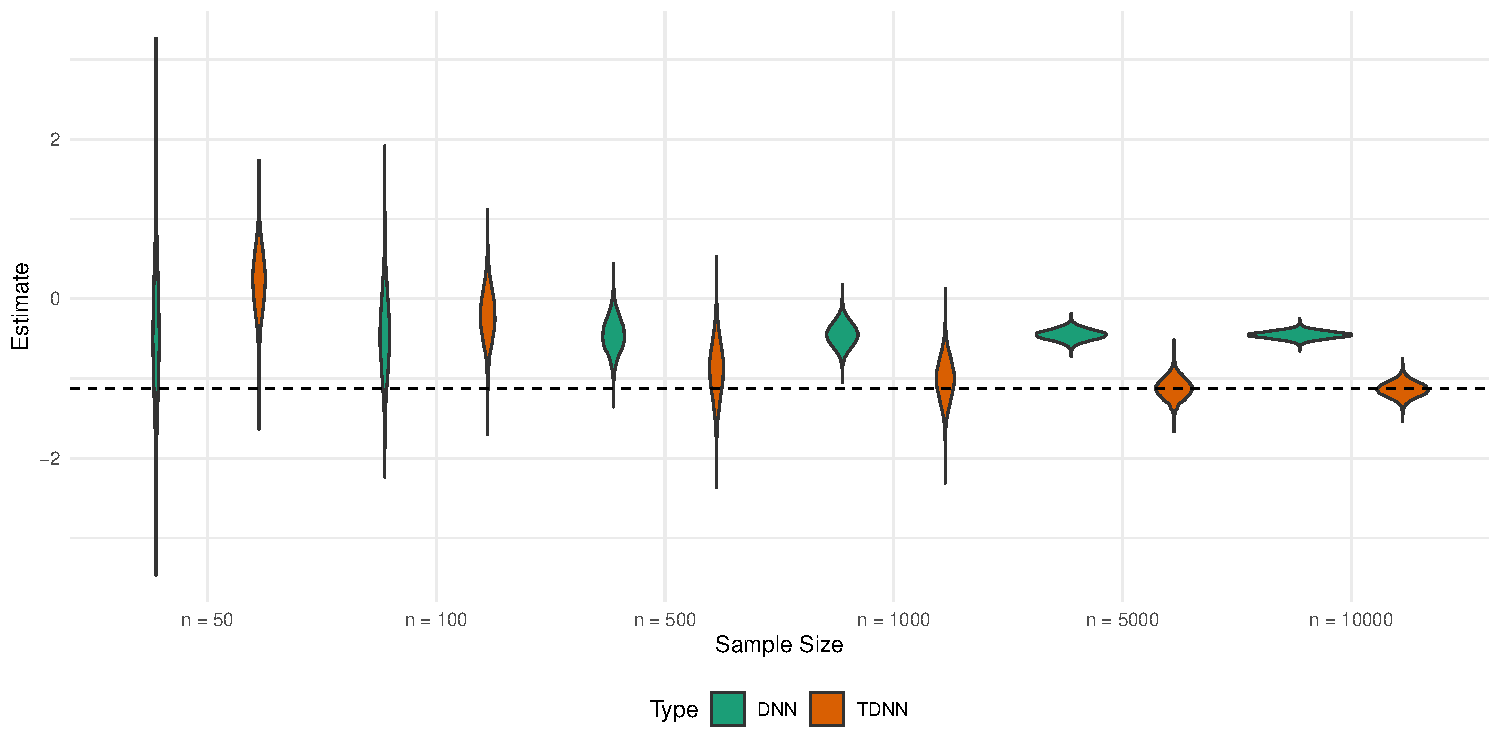
\includegraphics[width = \textwidth]{../Code/Simulations/Graphics/TDNN_DNN.pdf}
	\caption{Comparison of the DNN ($s = 20$) and TDNN ($s_1 = 20, s_2 = 50$) Estimators for different sample sizes.
		The dashed line indicates the value of the unknown regression function at the point of interest.
		Simulation Setup replicates Setting 1 from \citet{demirkaya_optimal_2024} for 10000 Monte Carlo Replications.}
\end{figure}

{\color{red} LOREM IPSUM}


\section{Application}\label{Application}
\hrule

\section{Conclusion}\label{Conclusion}
\hrule

\newpage
\printbibliography

\newpage
\appendix

\newpage
\section{Proofs for Results in Section \ref{sec:TDNN}}
\hrule

\newpage
\section{Proofs for Results in Section \ref{sec:pw_inf}}
\hrule

\subsection{Useful Lemmas for Proofs for Results in Section \ref{sec:pw_inf}}
\hrule

\begin{lem}[\citet{lee_u-statistics_2019} - Chapter 5, Theorem 1]\label{thm:lee_ch5_1}\mbox{}\\*
	Let $U_n$ be a U-statistic of degree $s$ based on a kernel $\psi_s$.
	Then, the Jackknife Variance estimator takes the following form.
	\begin{equation}
		\hat{\omega}^{2}_{JK}\left(\mathbf{x}; \mathbf{D}_n\right)
		= \frac{n-1}{n^2}\binom{n-1}{s}^{-2}\sum_{c = 0}^{s}\left(cn - s^2\right)S_c
	\end{equation}
	where the quantities $S_c$ are defined by
	\begin{equation}
		S_c
		= \sum_{\substack{\iota, \iota' \in L_{n,s}, \\ \, |\iota \cap \iota'| = c}}
		\psi_{s}(D_{\iota})\psi_{s}(D_{\iota'}).
	\end{equation}
\end{lem}

\subsection{Kernel (Conditional) Expectations}
\hrule

\begin{lem}[DNN Kernel Expecctation]\label{lem:DNN_k_exp}\mbox{}\\*
	Let $\mathbf{x}$ denote a point of interest.
	Then
	\begin{equation}
		\E_D\left[h_s\left(\mathbf{x}; D\right)\right]
		= \E_{1}\left[\mu\left(\mathbf{X}_1\right)\right].
	\end{equation}
\end{lem}

\begin{proof}[Proof of Lemma \ref{lem:DNN_k_exp}]
	\begin{equation}
		\begin{aligned}
			\E_D\left[h_s\left(\mathbf{x}; D\right)\right]
			 & = \E_D\left[\sum_{i = 1}^{s} \kappa\left(\mathbf{x}; \mathbf{Z}_i, D\right) Y_i\right]
			= s \E_{D}\left[\kappa\left(\mathbf{x}; \mathbf{Z}_1, D\right) Y_1\right]                 \\
			%
			 & = \E_{1}\left[\mu\left(\mathbf{X}_1\right) + \varepsilon_1\right]
			= \E_{1}\left[\mu\left(\mathbf{X}_1\right)\right].
		\end{aligned}
	\end{equation}
\end{proof}

\hrule

\begin{lem}[DNN Haj\'ek Kernel Expectation]\label{lem:psi_s_1}\mbox{}\\*
	Let $\mathbf{z}_1 = (\mathbf{x}_1, y_1)$ denote a specific realization of $\mathbf{Z}$ and $\mathbf{x}$ denote a point of interest.
	Then
	\begin{equation}
		\psi_{s}^{1}\left(\mathbf{x}; \mathbf{z}_1\right)
		= \varepsilon_1 \E_D\left[\kappa\left(\mathbf{x}; \mathbf{Z}_1, D\right)\, \Big| \, \mathbf{X}_1 = \mathbf{x}_1 \right]
		+ \E_{D}\left[\sum_{i = 1}^{s} \kappa\left(\mathbf{x}; \mathbf{Z}_i, D\right) \mu(\mathbf{X}_i)\, \Big| \, \mathbf{X}_1 = \mathbf{x}_1 \right]
	\end{equation}
\end{lem}

\begin{proof}[Proof of Lemma \ref{lem:psi_s_1}]
	\begin{equation}
		\begin{aligned}
			\psi_{s}^{1}\left(\mathbf{x}; \mathbf{z}_1\right)
			 & = \E_{D}\left[h_{s}\left(\mathbf{x}; D\right) \, | \, \mathbf{Z}_1 = \mathbf{z}_1 \right]
			= \E_{D}\left[\sum_{i = 1}^{s} \kappa\left(\mathbf{x}; \mathbf{Z}_i, D\right) Y_i \, \Big| \, \mathbf{Z}_1 = \mathbf{z}_1 \right]  \\
			%
			 & = \E_{D}\left[\left(\mu(\mathbf{x}_1) + \varepsilon_1\right)\kappa\left(\mathbf{x}; \mathbf{Z}_1, D\right)
			+ \sum_{i = 2}^{s} \kappa\left(\mathbf{x}; \mathbf{Z}_i, D\right) \mu(\mathbf{X}_i)\, \Big| \, \mathbf{Z}_1 = \mathbf{z}_1 \right] \\
			%
			 & = \varepsilon_1 \E_D\left[\kappa\left(\mathbf{x}; \mathbf{Z}_1, D\right)\, \Big| \, \mathbf{X}_1 = \mathbf{x}_1 \right]
			+ \E_{D}\left[\sum_{i = 1}^{s} \kappa\left(\mathbf{x}; \mathbf{Z}_i, D\right) \mu(\mathbf{X}_i)\, \Big| \, \mathbf{X}_1 = \mathbf{x}_1 \right]
		\end{aligned}
	\end{equation}
\end{proof}

\hrule

\begin{lem}[TDNN Haj\'ek Kernel Expectation]\label{lem:psi_s1s2_1}\mbox{}\\*
	Let $\mathbf{z}_1 = (\mathbf{x}_1, y_1)$ denote a specific realization of $\mathbf{Z}$ and $\mathbf{x}$ denote a point of interest.
	Let $D = \left\{\mathbf{Z}_1, \dotsc, \mathbf{Z}_{s_2} \right\}$ and $D' = \left\{\mathbf{Z}_1^{\prime}, \dotsc, \mathbf{Z}_{s_1}^{\prime} \right\}$ denote two independent and i.i.d. samples drawn from $P$.
	Furthermore, let $\mathbf{X} \sim P$ and $\mathbf{X} \indep D,D'$.
	Then
	\begin{equation}
		\begin{aligned}
			\psi_{s_1, s_2}^{1}\left(\mathbf{x}; \mathbf{z}_1\right)
			 & = w_{1}^{*} \left(
			\frac{s_2}{s_1}\left(\varepsilon_1 \E_{D'}\left[\kappa\left(\mathbf{x}; \mathbf{Z}_1^{\prime}, D'\right)\, \Big| \, \mathbf{X}_1^{\prime} = \mathbf{x}_1 \right]
				+ \E_{D'}\left[\sum_{i = 1}^{s} \kappa\left(\mathbf{x}; \mathbf{Z}_i^{\prime}, D'\right) \mu(\mathbf{X}_i^{\prime})\, \Big| \, \mathbf{X}_1 ^{\prime}= \mathbf{x}_1 \right]\right)
			+ \frac{s_2}{s_2 - s_1}\E\left[\mu(\mathbf{X})\right]\right)                                                                                          \\
			 & \quad + w_{2}^{*} \left(\varepsilon_1 \E_D\left[\kappa\left(\mathbf{x}; \mathbf{Z}_1, D\right)\, \Big| \, \mathbf{X}_1 = \mathbf{x}_1 \right]
			+ \E_{D}\left[\sum_{i = 1}^{s} \kappa\left(\mathbf{x}; \mathbf{Z}_i, D\right) \mu(\mathbf{X}_i)\, \Big| \, \mathbf{X}_1 = \mathbf{x}_1 \right]\right) \\
		\end{aligned}
	\end{equation}
\end{lem}

\begin{proof}[Proof of Lemma \ref{lem:psi_s1s2_1}]
	\begin{equation}
		\begin{aligned}
			\psi_{s_1, s_2}^{1}\left(\mathbf{x}; \mathbf{z}_1\right)
			 & = \E_{D}\left[w_{1}^{*} \tilde{\mu}_{s_1}\left(\mathbf{x}; D\right)
				+ w_{2}^{*} h_{s_2}\left(\mathbf{x}; D\right)\, | \, \mathbf{Z}_1 = \mathbf{z}_1\right]
			= \E_{D}\left[h_{s_1, s_2}\left(\mathbf{x}; D\right) \, | \, \mathbf{Z}_1 = \mathbf{z}_1 \right]                                                             \\
			%
			 & = w_{1}^{*} \E_{D}\left[\tilde{\mu}_{s_1}\left(\mathbf{x}; D\right)\, | \, \mathbf{Z}_1 = \mathbf{z}_1\right]
			+ w_{2}^{*} \E_D\left[h_{s_2}\left(\mathbf{x}; D\right)\, | \, \mathbf{Z}_1 = \mathbf{z}_1\right]                                                            \\
			%
			 & = w_{1}^{*} \E_{D}\left[\binom{s_2}{s_1}^{-1}\sum_{\ell \in L_{s_2, s_1}}h_{s_1}\left(\mathbf{x}; D_\ell\right)\, | \, \mathbf{Z}_1 = \mathbf{z}_1\right]
			+ w_{2}^{*} \E_D\left[h_{s_2}\left(\mathbf{x}; D\right)\, | \, \mathbf{Z}_1 = \mathbf{z}_1\right]                                                            \\
			%
			 & = w_{1}^{*} \binom{s_2}{s_1}^{-1}\left(\E_{D}\left[
				\sum_{\ell \in L_{s_1 - 1}\left([s_2]\backslash \{1\}\right)}h_{s_1}\left(\mathbf{x}; D_{\ell \cup 1}\right)
				\sum_{\ell \in L_{s_1}\left([s_2]\backslash \{1\}\right)}h_{s_1}\left(\mathbf{x}; D_\ell\right)
				\, | \, \mathbf{Z}_1 = \mathbf{z}_1\right]
			\right)                                                                                                                                                      \\
			 & \quad + w_{2}^{*} \E_D\left[h_{s_2}\left(\mathbf{x}; D\right)\, | \, \mathbf{Z}_1 = \mathbf{z}_1\right]                                                   \\
			%
			 & = w_{1}^{*} \binom{s_2}{s_1}^{-1}\left(
			\binom{s_2-1}{s_1-1}\E_{1:s_1}\left[h_{s_1}\left(\mathbf{x}; D_{[s_1]}\right) \, | \, \mathbf{Z}_1 = \mathbf{z}_1 \right]
			+ \binom{s_2-1}{s_1}\E_{2:(s_1+1)}\left[h_{s_1}\left(\mathbf{x}; D_{2:(s_1+1)}\right)\right]
			\right)                                                                                                                                                      \\
			 & \quad + w_{2}^{*} \E_D\left[h_{s_2}\left(\mathbf{x}; D\right)\, | \, \mathbf{Z}_1 = \mathbf{z}_1\right]                                                   \\
			%
			 & = w_{1}^{*} \binom{s_2}{s_1}^{-1}\left(
			\binom{s_2-1}{s_1-1}\psi_{s_1}^{1}\left(\mathbf{x}; \mathbf{z_1}\right)
			+ \binom{s_2-1}{s_1}\E_{2:(s_1+1)}\left[h_{s_1}\left(\mathbf{x}; D_{2:(s_1+1)}\right)\right]
			\right) + w_{2}^{*} \psi_{s_2}^{1}\left(\mathbf{x}; \mathbf{z_1}\right)
		\end{aligned}
	\end{equation}
	Using Lemmas \ref{lem:DNN_k_exp} and \ref{lem:psi_s_1}, we can further simplify this term significantly.
	\begin{equation}
		\begin{aligned}
			\psi_{s_1, s_2}^{1}\left(\mathbf{x}; \mathbf{z}_1\right)
			 & = w_{1}^{*} \left(\frac{s_2}{s_1}\psi_{s_1}^{1}\left(\mathbf{x}; \mathbf{z_1}\right)
			+ \frac{s_2}{s_2 - s_1}\E\left[\mu(\mathbf{X})\right]\right)
			+ w_{2}^{*} \psi_{s_2}^{1}\left(\mathbf{x}; \mathbf{z_1}\right)                                                                                       \\
			%
			 & = w_{1}^{*} \left(
			\frac{s_2}{s_1}\left(\varepsilon_1 \E_{D'}\left[\kappa\left(\mathbf{x}; \mathbf{Z}_1, D'\right)\, \Big| \, \mathbf{X}_1 = \mathbf{x}_1 \right]
				+ \E_{D'}\left[\sum_{i = 1}^{s} \kappa\left(\mathbf{x}; \mathbf{Z}_i, D'\right) \mu(\mathbf{X}_i)\, \Big| \, \mathbf{X}_1 = \mathbf{x}_1 \right]\right)
			+ \frac{s_2}{s_2 - s_1}\E\left[\mu(\mathbf{X})\right]\right)                                                                                          \\
			 & \quad + w_{2}^{*} \left(\varepsilon_1 \E_D\left[\kappa\left(\mathbf{x}; \mathbf{Z}_1, D\right)\, \Big| \, \mathbf{X}_1 = \mathbf{x}_1 \right]
			+ \E_{D}\left[\sum_{i = 1}^{s} \kappa\left(\mathbf{x}; \mathbf{Z}_i, D\right) \mu(\mathbf{X}_i)\, \Big| \, \mathbf{X}_1 = \mathbf{x}_1 \right]\right) \\
			%
			 & \quad = {\color{red} LOREM IPSUM}
		\end{aligned}
	\end{equation}
\end{proof}

\newpage
\subsection{Kernel Variances \& Covariances}
\hrule

\begin{lem}[\citet{demirkaya_optimal_2024} - Lemma 12]\label{lem:dem12}\mbox{}\\*
	Let $D = \{\mathbf{Z}_1, \dotsc, \mathbf{Z}_s\}$ an i.i.d. sample drawn from $P$.
	The indicator functions $\kappa\left(\mathbf{x}; \mathbf{Z}_i, D\right)$ satisfy the following properties.
	\begin{enumerate}
		\item For any $i \neq j$, we have $\kappa\left(\mathbf{x}; \mathbf{Z}_i, D\right) \kappa\left(\mathbf{x}; \mathbf{Z}_j, D\right)=0$ with probability one;
		\item $\sum_{i=1}^{s} \kappa\left(\mathbf{x}; \mathbf{Z}_i, D\right)=1$;
		\item $\forall i \in [s]: \quad \mathbb{E}_{1:s}\left[\kappa\left(\mathbf{x}; \mathbf{Z}_i, D\right)\right]=s^{-1}$
		\item $\mathbb{E}_{2: s}\left[\kappa\left(\mathbf{x}; \mathbf{Z}_1, D\right)\right]=\left\{1-\varphi\left(B\left(\mathbf{x},\left\|\mathbf{X}_1-\mathbf{x}\right\|\right)\right)\right\}^{s-1}$
	\end{enumerate}
	Here $\mathbb{E}_{i: s}$ denotes the expectation with respect to $\left\{\mathbf{Z}_i, \mathbf{Z}_{i+1}, \cdots, \mathbf{Z}_s\right\}$.
	Furthermore, $\varphi$ denotes the probability measure on $\mathbb{R}^{d}$ induced by the random vector $\mathbf{X}$.
\end{lem}

\hrule

\begin{lem}[\citet{demirkaya_optimal_2024} - Lemma 13]\label{lem:dem13}\mbox{}\\*
	For any $L^1$ function $f$ that is continuous at $\mathbf{x}$, it holds that
	\begin{equation}
		\lim _{s \rightarrow \infty} \E_1\left[f\left(\mathbf{X}_1\right) s \E_{2: s}\left[\kappa(\mathbf{x}; \mathbf{Z}_1, D)\right]\right]
		= f(\mathbf{x}).
	\end{equation}
\end{lem}

\hrule

\begin{lem}[Adapted from \citet{demirkaya_optimal_2024}]\label{lem:omega_s}\mbox{}\\*
	Let $D = \{\mathbf{Z}_1, \dotsc, \mathbf{Z}_{s}\}$ be a vector of i.i.d. random variables drawn from $P$.
	Furthermore, let
	\begin{equation}
		\Omega_{s}
		= \E\left[h_{s}^{2}\left(\mathbf{x}; \mathbf{Z}_1, \ldots,  \mathbf{Z}_{s}\right)\right].
	\end{equation}
	Then,
	\begin{equation}
		\Omega_{s}
		= \E_1\left[\mu^2\left(\mathbf{X}_1\right) s \E_{2:s}\left[\kappa\left(\mathbf{x}; \mathbf{Z}_1, D\right)\right]\right] + \sigma_{\varepsilon}^2
		\lesssim \mu^2(\mathbf{x}) + \sigma_{\varepsilon}^2 + o(1)
		\quad \text{as} \quad s \rightarrow \infty.
	\end{equation}
\end{lem}


\newpage
\begin{lem}\label{lem:omega_sc}\mbox{}\\*
	Let $D = \{\mathbf{Z}_1, \dotsc, \mathbf{Z}_{s}\}$ be a vector of i.i.d. random variables drawn from $P$.
	Let $D^{\prime} = \{\mathbf{Z}_1, \dotsc, \mathbf{Z}_{c}, \mathbf{Z}_{c+1}^{\prime}, \dotsc,  \mathbf{Z}_{s}^{\prime}\}$ where $\mathbf{Z}_{c+1}^{\prime}, \dotsc,  \mathbf{Z}_{s}^{\prime}$ are i.i.d. draws from $P$ that are independent of $D$.
	Furthermore, let
	\begin{equation}
		\Omega_{s}^{c}
		= \E\left[h_{s}\left(\mathbf{x}; \mathbf{Z}_1, \ldots, \mathbf{Z}_{c}, \mathbf{Z}_{c+1}, \ldots, \mathbf{Z}_{s}\right) \cdot
			h_{s}\left(\mathbf{x}; \mathbf{Z}_1, \ldots,\mathbf{Z}_{c}, \mathbf{Z}_{c+1}^{\prime}, \ldots, \mathbf{Z}_{s}^{\prime}\right)\right].
	\end{equation}
	Then,
	\begin{equation}
		\Omega_{s}^{c}
		\lesssim \frac{s^2 + cs  - c^2}{s^2} \mu^2(\mathbf{x}) + (c/s) \sigma_{\varepsilon}^2 + o(1)
		\quad \text{for} \quad s \quad \text{sufficiently large}
	\end{equation}
	and thus
	\begin{equation}
		\Omega_{s}^{c}
		\lesssim \mu^2(\mathbf{x}) + o(1)
		\quad \text{as} \quad s \rightarrow \infty.
	\end{equation}
\end{lem}

\begin{proof}[Proof of Lemma \ref{lem:omega_sc}]
	\begin{equation}
		\begin{aligned}
			\Omega_{s}^{c}
			 & = \E\left[h_{s}\left(\mathbf{x}; \mathbf{Z}_1, \ldots, \mathbf{Z}_{c}, \mathbf{Z}_{c+1}, \ldots, \mathbf{Z}_{s}\right) \cdot
			h_{s}\left(\mathbf{x}; \mathbf{Z}_1, \ldots,\mathbf{Z}_{c}, \mathbf{Z}_{c+1}^{\prime}, \ldots, \mathbf{Z}_{s}^{\prime}\right)\right]                                                                \\
			%
			 & = \E_{D, D'}\left[
				\left(\sum_{i = 1}^{s}\kappa\left(\mathbf{x}; \mathbf{Z}_{i}, D\right)Y_{i}\right)
				\left(\sum_{j = 1}^{c}\kappa\left(\mathbf{x}; \mathbf{Z}_{j}, D^{\prime}\right)Y_{j}
				+ \sum_{j = c+1}^{s}\kappa\left(\mathbf{x}; \mathbf{Z}_{j}^{\prime}, D^{\prime}\right)Y_{j}^{\prime}\right)
			\right]                                                                                                                                                                                             \\
			%
			 & = \E_{D, D'}\left[\sum_{i = 1}^{c}\sum_{j = 1}^{c}\kappa\left(\mathbf{x}; \mathbf{Z}_{i}, D\right)\kappa\left(\mathbf{x}; \mathbf{Z}_{j}, D^{\prime}\right)Y_{i}Y_{j}\right]
			+  \E_{D, D'}\left[\sum_{i = 1}^{c}\sum_{j = c+1}^{s}\kappa\left(\mathbf{x}; \mathbf{Z}_{i}, D\right)\kappa\left(\mathbf{x}; \mathbf{Z}_{j}^{\prime}, D^{\prime}\right)Y_{i}Y_{j}^{\prime}\right]   \\
			 & \quad + \E_{D, D'}\left[\sum_{i = c+1}^{s}\sum_{j = 1}^{c}\kappa\left(\mathbf{x}; \mathbf{Z}_{i}, D\right)\kappa\left(\mathbf{x}; \mathbf{Z}_{j}, D^{\prime}\right)Y_{i}Y_{j}\right]
			+  \E_{D, D'}\left[\sum_{i = c+1}^{s}\sum_{j = c+1}^{s}\kappa\left(\mathbf{x}; \mathbf{Z}_{i}, D\right)\kappa\left(\mathbf{x}; \mathbf{Z}_{j}^{\prime}, D^{\prime}\right)Y_{i}Y_{j}^{\prime}\right] \\
			%
			 & = \E_{D, D'}\left[c \kappa\left(\mathbf{x}; \mathbf{Z}_{1}, D\right)\kappa\left(\mathbf{x}; \mathbf{Z}_{1}, D^{\prime}\right)Y_{1}^{2}\right]
			+ \E_{D, D'}\left[c(s-c) \kappa\left(\mathbf{x}; \mathbf{Z}_{1}, D\right)\kappa\left(\mathbf{x}; \mathbf{Z}_{c+1}^{\prime}, D^{\prime}\right)Y_{1}Y_{c+1}^{\prime}\right]                           \\
			 & \quad + \E_{D, D'}\left[c(s-c) \kappa\left(\mathbf{x}; \mathbf{Z}_{c+1}, D\right)\kappa\left(\mathbf{x}; \mathbf{Z}_{1}, D^{\prime}\right)Y_{c+1}Y_{1}\right]                                    \\
			 & \quad + \E_{D, D'}\left[(s-c)^2 \kappa\left(\mathbf{x}; \mathbf{Z}_{c+1}, D\right)\kappa\left(\mathbf{x}; \mathbf{Z}_{c+1}^{\prime}, D^{\prime}\right)Y_{c+1}Y_{c+1}^{\prime}\right]
		\end{aligned}
	\end{equation}
	Starting from this decomposition, we will analyze the terms one by one.
	First, by honesty and an application of Lemma \ref{lem:dem12}, we find the following.
	\begin{equation}
		\begin{aligned}
			\E_{D, D'}\left[c\kappa\left(\mathbf{x}; \mathbf{Z}_{1}, D\right)\kappa\left(\mathbf{x}; \mathbf{Z}_{1}, D^{\prime}\right)Y_{1}^{2}\right]
			 & = \E_{D, D'}\left[c\kappa\left(\mathbf{x}; \mathbf{Z}_{1}, D\right)\kappa\left(\mathbf{x}; \mathbf{Z}_{1}, D^{\prime}\right)\left(\mu^2(\mathbf{X}_1) + \sigma_{\varepsilon}^{2}\right)\right]                   \\
			%
			 & = \E_{1}\left[\left(\mu^2(\mathbf{X}_1) + \sigma_{\varepsilon}^{2}\right) c\E_{2:s}\left[\kappa\left(\mathbf{x}; \mathbf{Z}_{1}, D\right)\kappa\left(\mathbf{x}; \mathbf{Z}_{1}, D^{\prime}\right)\right]\right] \\
			%
			 & = \E_{1}\left[\left(\mu^2(\mathbf{X}_1) + \sigma_{\varepsilon}^{2}\right) c\left\{1 - \varphi\left(B\left(\mathbf{x}, \|\mathbf{X}_1 - \mathbf{x}\|\right)\right)\right\}^{2s-c-1}\right]                        \\
			%
			 & \leq (c/s) \E_{1}\left[\left(\mu^2(\mathbf{X}_1) + \sigma_{\varepsilon}^{2}\right) s\left\{1 - \varphi\left(B\left(\mathbf{x}, \|\mathbf{X}_1 - \mathbf{x}\|\right)\right)\right\}^{s-1}\right]                  \\
			%
			 & \lesssim (c/s)\left(\mu^2(\mathbf{x}) + \sigma_{\varepsilon}\right) + o(1)
		\end{aligned}
	\end{equation}
	Similarly, we can find that:
	\begin{equation}
		\begin{aligned}
			 & \E_{D, D'}\left[c(s-c) \kappa\left(\mathbf{x}; \mathbf{Z}_{1}, D\right)\kappa\left(\mathbf{x}; \mathbf{Z}_{c+1}^{\prime}, D^{\prime}\right)Y_{1}Y_{c+1}^{\prime}\right]                                          \\
			%
			 & \quad = \E_{D, D'}\left[\mu(\mathbf{X}_1)\mu(\mathbf{X}_{c+1}^{\prime}) \, c(s-c) \, \kappa\left(\mathbf{x}; \mathbf{Z}_{1}, D\right)\kappa\left(\mathbf{x}; \mathbf{Z}_{c+1}^{\prime}, D^{\prime}\right)\right] \\
			%
			 & \quad \leq \E_{D}\left[|\mu(\mathbf{X}_1)| \, c \, \kappa\left(\mathbf{x}; \mathbf{Z}_{1}, D\right)\right]
			\E_{D'}\left[|\mu(\mathbf{X}_{c+1}^{\prime})| \, (s-c) \, \kappa\left(\mathbf{x}; \mathbf{Z}_{c+1}^{\prime}, D^{\prime}\right)\right]                                                                               \\
			% 
			 & \quad = \frac{c (s-c)}{s^2} \leq \E_{D}\left[|\mu(\mathbf{X}_1)| \, s \, \kappa\left(\mathbf{x}; \mathbf{Z}_{1}, D\right)\right]
			\E_{D'}\left[|\mu(\mathbf{X}_{c+1}^{\prime})| \, s \, \kappa\left(\mathbf{x}; \mathbf{Z}_{c+1}^{\prime}, D^{\prime}\right)\right]                                                                                   \\
			%
			 & \quad = \frac{c (s-c)}{s^2} \left(\E_{D}\left[|\mu(\mathbf{X}_1)| \, s \, \kappa\left(\mathbf{x}; \mathbf{Z}_{1}, D\right)\right]\right)^2                                                                       \\
			% 
			 & \quad = \frac{c (s-c)}{s^2} \left(\E_{1}\left[|\mu(\mathbf{X}_1)| s\left\{1 - \varphi\left(B\left(\mathbf{x}, \|\mathbf{X}_1 - \mathbf{x}\|\right)\right)\right\}^{s-1}\right]\right)^2                          \\
			%
			 & \quad \lesssim \frac{c(s-c)}{s^2}\mu^2(\mathbf{x}) + o(1)
		\end{aligned}
	\end{equation}
	Following analogous steps, we find the same result for the third term.
	\begin{equation}
		\begin{aligned}
			\E_{D, D'}\left[c(s-c) \kappa\left(\mathbf{x}; \mathbf{Z}_{c+1}, D\right)\kappa\left(\mathbf{x}; \mathbf{Z}_{1}, D^{\prime}\right)Y_{c+1}Y_{1}\right]
			\lesssim \frac{c(s-c)}{s^2}\mu^2(\mathbf{x}) + o(1)
		\end{aligned}
	\end{equation}
	The fourth term can be asymptotically bounded in the following way.
	\begin{equation}
		\begin{aligned}
			 & \E_{D, D'}\left[(s-c)^2 \kappa\left(\mathbf{x}; \mathbf{Z}_{c+1}, D\right)\kappa\left(\mathbf{x}; \mathbf{Z}_{c+1}^{\prime}, D^{\prime}\right)Y_{c+1}Y_{c+1}^{\prime}\right]                                           \\
			%
			 & \quad = \E_{D, D'}\left[\mu(\mathbf{X}_{c+1})\mu(\mathbf{X}_{c+1}^{\prime})\, (s-c)^2 \, \kappa\left(\mathbf{x}; \mathbf{Z}_{c+1}, D\right)\kappa\left(\mathbf{x}; \mathbf{Z}_{c+1}^{\prime}, D^{\prime}\right)\right] \\
			%
			 & \quad \leq \E_{D}\left[|\mu(\mathbf{X}_{c+1})|\, (s-c) \, \kappa\left(\mathbf{x}; \mathbf{Z}_{c+1}, D\right)\right]
			\E_{D'}\left[|\mu(\mathbf{X}_{c+1}^{\prime})|\, (s-c) \, \kappa\left(\mathbf{x}; \mathbf{Z}_{c+1}^{\prime}, D^{\prime}\right)\right]                                                                                      \\
			%
			 & \quad = \frac{(s-c)^2}{s^2} \E_{D}\left[|\mu(\mathbf{X}_{c+1})|\, s \, \kappa\left(\mathbf{x}; \mathbf{Z}_{c+1}, D\right)\right]
			\E_{D'}\left[|\mu(\mathbf{X}_{c+1}^{\prime})|\, s \, \kappa\left(\mathbf{x}; \mathbf{Z}_{c+1}^{\prime}, D^{\prime}\right)\right]                                                                                          \\
			%
			 & \quad = \frac{(s-c)^2}{s^2} \left(\E_{D}\left[|\mu(\mathbf{X}_{c+1})|\, s \, \kappa\left(\mathbf{x}; \mathbf{Z}_{c+1}, D\right)\right]\right)^2                                                                        \\
			%
			 & \quad \lesssim \frac{(s-c)^2}{s^2}\mu^2(\mathbf{x}) + o(1)
		\end{aligned}
	\end{equation}
	The result of Lemma \ref{lem:omega_sc} follows immediately.
\end{proof}

\newpage
\begin{lem}\label{lem:upsilon_s}\mbox{}\\*
	Let $D = \{\mathbf{Z}_1, \dotsc, \mathbf{Z}_{s_2}\}$ be a vector of i.i.d. random variables drawn from $P$ for $s_2 > s_1$.
	Furthermore, let
	\begin{equation}
		\Upsilon_{s_1, s_2}
		= \E\left[h_{s_1}\left(\mathbf{x}; \mathbf{Z}_1, \ldots,  \mathbf{Z}_{s_1}\right) \cdot
			h_{s_2}\left(\mathbf{x}; \mathbf{Z}_1, \ldots,\mathbf{Z}_{s_1}, \ldots, \mathbf{Z}_{s_2}\right)\right].
	\end{equation}
	Then,
	\begin{equation}
		\Upsilon_{s_1, s_2}
		\lesssim \mu^{2}\left(\mathbf{x}\right) + \sigma^2_{\varepsilon} + o(1)
		\quad \text{as} \quad s_1, s_2 \rightarrow \infty
		\quad \text{with} \quad
		0 < c_1 \leq s_1 / s_2 \leq c_2 < 1.
	\end{equation}
\end{lem}

\begin{proof}[Proof of Lemma \ref{lem:upsilon_s}]
	\begin{equation}
		\begin{aligned}
			\Upsilon_{s_1, s_2}
			 & = \E\left[h_{s_1}\left(\mathbf{x}; \mathbf{Z}_1, \ldots,  \mathbf{Z}_{s_1}\right) \cdot
			h_{s_2}\left(\mathbf{x}; \mathbf{Z}_1, \ldots,\mathbf{Z}_{s_1}, \ldots, \mathbf{Z}_{s_2}\right)\right]                                                                             \\
			%
			 & = \E_{D}\left[
				\left(\sum_{i = 1}^{s_1} \kappa(\mathbf{x}; \mathbf{Z}_i, D_{[s_1]})Y_i\right)
				\left(\sum_{j = 1}^{s_1}\kappa(\mathbf{x}; \mathbf{Z}_j, D)Y_j + \sum_{j = s_1 + 1}^{s_2}\kappa(\mathbf{x}; \mathbf{Z}_j, D)Y_j\right)
			\right]                                                                                                                                                                            \\
			%
			 & = \E_{D}\left[\sum_{i = 1}^{s_1} \kappa(\mathbf{x}; \mathbf{Z}_i, D) Y_i^2\right]
			+ \E_{D}\left[\sum_{i = 1}^{s_1}\sum_{j = s_1 + 1}^{s_2}\kappa(\mathbf{x}; \mathbf{Z}_i, D_{[s_1]})\kappa(\mathbf{x}; \mathbf{Z}_j, D) Y_i Y_j\right]                              \\
			%
			 & = \E_{D}\left[Y_1^2 \, s_1 \, \kappa(\mathbf{x}; \mathbf{Z}_1, D)\right]
			+ \E_{D}\left[Y_{1} Y_{s_2} \, s_1 (s_2 - s_1) \, \kappa(\mathbf{x}; \mathbf{Z}_1, D_{[s_1]})\kappa(\mathbf{x}; \mathbf{Z}_{s_2}, D)\right]                                        \\
			%
			 & = \E_{D}\left[\left(\mu^2(\mathbf{X}_1) + \sigma^2_{\varepsilon}\right) \, s_1 \, \kappa(\mathbf{x}; \mathbf{Z}_1, D)\right]
			+ \E_{D}\left[\mu(\mathbf{X}_1) \mu(\mathbf{X}_{s_2}) \, s_1 (s_2 - s_1) \, \kappa(\mathbf{x}; \mathbf{Z}_1, D_{[s_1]})\kappa(\mathbf{x}; \mathbf{Z}_{s_2}, D)\right]              \\
			%
			 & = \frac{s_1}{s_2}\E_{D}\left[\left(\mu^2(\mathbf{X}_1) + \sigma^2_{\varepsilon}\right) \, s_1 \, \kappa(\mathbf{x}; \mathbf{Z}_1, D)\right]
			+ \frac{s_2 - s_1}{s_2}\E_{D}\left[\mu(\mathbf{X}_1) \mu(\mathbf{X}_{s_2}) \, s_1 s_2 \, \kappa(\mathbf{x}; \mathbf{Z}_1, D_{[s_1]})\kappa(\mathbf{x}; \mathbf{Z}_{s_2}, D)\right] \\
			%
			 & \leq \frac{s_1}{s_2} \E_{D}\left[\left(\mu^2(\mathbf{X}_1) + \sigma^2_{\varepsilon}\right) \, s_2 \, \kappa(\mathbf{x}; \mathbf{Z}_1, D)\right]                                 \\
			 & \quad \quad + \frac{s_2 - s_1}{s_2}\E_{D}\left[|\mu(\mathbf{X}_1)| \, s_1 \, \kappa(\mathbf{x}; \mathbf{Z}_1, D_{[s_1]})\right]
			\E_{D}\left[|\mu(\mathbf{X}_{s_2})| \, s_2 \, \kappa(\mathbf{x}; \mathbf{Z}_{s_2}, D)\right]                                                                                       \\
			%
			 & \lesssim \mu^{2}\left(\mathbf{x}\right) + \sigma^2_{\varepsilon} + o(1).
		\end{aligned}
	\end{equation}
\end{proof}

\hrule

\begin{lem}\label{lem:upsilon_sc}\mbox{}\\*
	Let $D = \{\mathbf{Z}_1, \dotsc, \mathbf{Z}_{s_2}\}$ be a vector of i.i.d. random variables drawn from $P$ for $s_2 > s_1$.
	Let $D^{\prime} = \{\mathbf{Z}_1, \dotsc, \mathbf{Z}_{c}, \mathbf{Z}_{c+1}^{\prime}, \dotsc,  \mathbf{Z}_{s_1}^{\prime}\}$ where $\mathbf{Z}_{c+1}^{\prime}, \dotsc,  \mathbf{Z}_{s_1}^{\prime}$ are i.i.d. draws from $P$ that are independent of $D$.
	Furthermore, let
	\begin{equation}
		\Upsilon_{s_1, s_2}^{c}
		= \E\left[h_{s_1}\left(\mathbf{x}; \mathbf{Z}_1, \ldots, \mathbf{Z}_c, \mathbf{Z}^{\prime}_{c+1}, \ldots,  \mathbf{Z}^{\prime}_{s_1}\right) \cdot
			h_{s_2}\left(\mathbf{x}; \mathbf{Z}_1, \ldots, \mathbf{Z}_{s_2}\right)\right].
	\end{equation}
	Then,
	\begin{equation}
		\begin{aligned}
			 & \Upsilon_{s_1, s_2}^{c}
			\lesssim \frac{c s_2 - c^2 + s_1 s_2}{s_1 s_2}\mu^2(\mathbf{x}) + (c/s_1) \sigma^2_{\varepsilon} + o(1) \\
			%
			 & \text{for} \quad s_1, s_2 \quad \text{sufficiently large}
			\quad \text{with} \quad
			0 < c_1 \leq s_1 / s_2 \leq c_2 < 1
		\end{aligned}
	\end{equation}
	and thus
	\begin{equation}
		\Upsilon_{s_1, s_2}^{c}
		\lesssim \mu^2(\mathbf{x}) + o(1)
		\quad \text{as} \quad s_1, s_2 \rightarrow \infty
		\quad \text{with} \quad
		0 < c_1 \leq s_1 / s_2 \leq c_2 < 1.
	\end{equation}
\end{lem}

\begin{proof}[Proof of Lemma \ref{lem:upsilon_sc}]
	\begin{equation}
		\begin{aligned}
			\Upsilon_{s_1, s_2}^{c}
			 & = \E\left[h_{s_1}\left(\mathbf{x}; \mathbf{Z}_1, \ldots, \mathbf{Z}_c, \mathbf{Z}^{\prime}_{c+1}, \ldots,  \mathbf{Z}^{\prime}_{s_1}\right) \cdot
			h_{s_2}\left(\mathbf{x}; \mathbf{Z}_1, \ldots, \mathbf{Z}_{s_2}\right)\right]                                                                                                    \\
			%                                                                     
			 & = \E_{D, D'}\left[
				\left(\sum_{i = 1}^{c} \kappa(\mathbf{x}; \mathbf{Z}_i, D^{\prime})Y_i + \sum_{i = c+1}^{s_1} \kappa(\mathbf{x}; \mathbf{Z}_i^{\prime}, D^{\prime})Y_i^{\prime}\right)
				\left(\sum_{j = 1}^{c} \kappa(\mathbf{x}; \mathbf{Z}_j, D)Y_j + \sum_{j = c+1}^{s_2}\kappa(\mathbf{x}; \mathbf{Z}_j, D)Y_j \right)
			\right]                                                                                                                                                                          \\
			%
			 & = \E_{D, D'}\left[\sum_{i = 1}^{c}\sum_{j = 1}^{c} \kappa(\mathbf{x}; \mathbf{Z}_i, D^{\prime})\kappa(\mathbf{x}; \mathbf{Z}_j, D)Y_i Y_j\right]
			+ \E_{D, D'}\left[\left(\sum_{i = 1}^{c}\kappa(\mathbf{x}; \mathbf{Z}_i, D^{\prime}) Y_i\right) \left(\sum_{j = c+1}^{s_2} \kappa(\mathbf{x}; \mathbf{Z}_j, D) Y_j\right)\right] \\
			 & \quad + \E_{D, D'}\left[\sum_{i = c+1}^{s_1}\sum_{j = 1}^{c} \kappa(\mathbf{x}; \mathbf{Z}_i^{\prime}, D^{\prime})\kappa(\mathbf{x}; \mathbf{Z}_j, D)Y_i^{\prime} Y_j\right]
			+ \E_{D, D'}\left[\left(\sum_{i = c+1}^{s_1}\kappa(\mathbf{x}; \mathbf{Z}_i^{\prime}, D^{\prime}) Y_i^{\prime}\right)
				\left(\sum_{j = c+1}^{s_2} \kappa(\mathbf{x}; \mathbf{Z}_j, D) Y_j\right)\right]
		\end{aligned}
	\end{equation}
	Again, we have four terms to analyze individually.
	\begin{equation}
		\begin{aligned}
			\E_{D, D'}\left[\sum_{i = 1}^{c}\sum_{j = 1}^{c} \kappa(\mathbf{x}; \mathbf{Z}_i, D^{\prime})\kappa(\mathbf{x}; \mathbf{Z}_j, D)Y_i Y_j\right]
			 & = \E_{D, D'}\left[\sum_{i = 1}^{c} Y_{i}^2 \kappa(\mathbf{x}; \mathbf{Z}_i, D^{\prime})\kappa(\mathbf{x}; \mathbf{Z}_i, D)\right]                                                            \\
			%
			 & = \E_{D, D'}\left[Y_{1}^2 \, c \, \kappa(\mathbf{x}; \mathbf{Z}_1, D^{\prime})\kappa(\mathbf{x}; \mathbf{Z}_1, D)\right]                                                                     \\
			%
			 & = \E_{D, D'}\left[\left(\mu^2(\mathbf{X}_{1}) + \sigma^2_{\varepsilon}\right) \, c \, \kappa(\mathbf{x}; \mathbf{Z}_1, D_{[c]})\kappa(\mathbf{x}; \mathbf{Z}_1, D^{\prime}_{c+1:s_1})\right] \\
			%
			 & = \E_{D}\left[\left(\mu^2(\mathbf{X}_{1}) + \sigma^2_{\varepsilon}\right) \, c \, \kappa(\mathbf{x}; \mathbf{Z}_1, D)\right]                                                                 \\
			%
			 & = \frac{c}{s_1} \E_{D}\left[\left(\mu^2(\mathbf{X}_{1}) + \sigma^2_{\varepsilon}\right) \, s_1 \, \kappa(\mathbf{x}; \mathbf{Z}_1, D)\right]                                                 \\
			%
			 & \lesssim (c/s_1)(\mu^2(\mathbf{x}) + \sigma^2_{\varepsilon}) + o(1)
		\end{aligned}
	\end{equation}
	Considering the second term, we find the following.
	\begin{equation}
		\begin{aligned}
			 & \E_{D, D'}\left[\left(\sum_{i = 1}^{c}\kappa(\mathbf{x}; \mathbf{Z}_i, D^{\prime}) Y_i\right)
			\left(\sum_{j = c+1}^{s_2} \kappa(\mathbf{x}; \mathbf{Z}_j, D) Y_j\right)\right]                                                                                          \\                                                                                                                                                                         \\
			%
			 & \quad = \E_{D, D'}\left[\sum_{i = 1}^{c}\sum_{j = c+1}^{s_2}Y_i Y_j \kappa(\mathbf{x}; \mathbf{Z}_i, D^{\prime})\kappa(\mathbf{x}; \mathbf{Z}_j, D)\right]             \\
			%
			 & \quad = \E_{D, D'}\left[c(s_2 - c) \, Y_1 Y_{s_1} \kappa(\mathbf{x}; \mathbf{Z}_1, D^{\prime})\kappa(\mathbf{x}; \mathbf{Z}_{s_2}, D)\right]                           \\
			%
			 & \quad = \frac{c (s_2 - c)}{s_1 s_2}\E_{D, D'}\left[Y_1 Y_{s_2} \, s_1 s_2 \,\kappa(\mathbf{x}; \mathbf{Z}_1, D^{\prime})\kappa(\mathbf{x}; \mathbf{Z}_{s_2}, D)\right] \\
			%
			 & \quad \leq \frac{c (s_2 - c)}{s_1 s_2}
			\E_{D'}\left[|\mu(\mathbf{X}_1)| \, s_1  \,\kappa(\mathbf{x}; \mathbf{Z}_1, D^{\prime})\right]
			\E_{D}\left[|\mu(\mathbf{X}_{s_2})| \, s_2  \,\kappa(\mathbf{x}; \mathbf{Z}_{s_2}, D)\right]                                                                              \\
			%
			 & \quad \lesssim \frac{c(s_2 - c)}{s_1 s_2} \mu^2(\mathbf{x}) + o(1)
		\end{aligned}
	\end{equation}
	Similarly, by simplifying the third term, we find the following.
	\begin{equation}
		\begin{aligned}
			 & \E_{D, D'}\left[\sum_{i = c+1}^{s_1}\sum_{j = 1}^{c} \kappa(\mathbf{x}; \mathbf{Z}_i^{\prime}, D^{\prime})\kappa(\mathbf{x}; \mathbf{Z}_j, D)Y_i^{\prime} Y_j\right]                                                \\
			%
			 & \quad = \E_{D, D'}\left[Y_{s_1}^{\prime} Y_{1} \, (s_1 - c)c \, \kappa(\mathbf{x}; \mathbf{Z}_{s_1}^{\prime}, D^{\prime})\kappa(\mathbf{x}; \mathbf{Z}_1, D)\right]                                                 \\
			% 
			 & \quad = \frac{(s_1 - c)c}{s_1 s_2}\E_{D, D'}\left[\mu(\mathbf{X}_{s_1}^{\prime})\mu(\mathbf{X}_1) \, s_1 s_2 \, \kappa(\mathbf{x}; \mathbf{Z}_{s_1}^{\prime}, D^{\prime})\kappa(\mathbf{x}; \mathbf{Z}_1, D)\right] \\
			%
			 & \quad \leq \frac{(s_1 - c)c}{s_1 s_2}
			\E_{D}\left[|\mu(\mathbf{X}_{s_1}^{\prime})| \, s_1 \, \kappa(\mathbf{x}; \mathbf{Z}_{s_1}^{\prime}, D^{\prime})\right]
			\E_{D}\left[|\mu(\mathbf{X}_1)| \, s_2 \, \kappa(\mathbf{x}; \mathbf{Z}_1, D)\right]                                                                                                                                   \\
			%
			 & \quad \lesssim \frac{(s_1 - c)c}{s_1 s_2} \mu^2(\mathbf{x}) + o(1)
		\end{aligned}
	\end{equation}
	Lastly, concerning the fourth term, observe the following.
	\begin{equation}
		\begin{aligned}
			 & \E_{D, D'}\left[\left(\sum_{i = c+1}^{s_1}\kappa(\mathbf{x}; \mathbf{Z}_i^{\prime}, D^{\prime}) Y_i^{\prime}\right)
			\left(\sum_{j = c+1}^{s_2} \kappa(\mathbf{x}; \mathbf{Z}_j, D) Y_j\right)\right]                                                                                                                                                         \\
			%
			 & \quad = \E_{D, D'}\left[\sum_{i = c+1}^{s_1}\sum_{j = c+1}^{s_2}\kappa(\mathbf{x}; \mathbf{Z}_i^{\prime}, D^{\prime}) \kappa(\mathbf{x}; \mathbf{Z}_j, D)  Y_i^{\prime}Y_j\right]                                                     \\
			%
			 & \quad = \E_{D, D'}\left[\mu(\mathbf{X}_{s_1}^{\prime}) \mu(\mathbf{X}_{s_2}) \, (s_1 - c)(s_2 -c) \,\kappa(\mathbf{x}; \mathbf{Z}_{s_1}^{\prime}, D^{\prime}) \kappa(\mathbf{x}; \mathbf{Z}_{s_2}, D)  \right]                        \\                                                                                                                                                                       \\
			%
			 & \quad = \frac{(s_1 - c)(s_2 -c)}{s_1 s_2}\E_{D, D'}\left[\mu(\mathbf{X}_{s_1}^{\prime}) \mu(\mathbf{X}_{s_2}) \, s_1 s_2 \,\kappa(\mathbf{x}; \mathbf{Z}_{s_1}^{\prime}, D^{\prime}) \kappa(\mathbf{x}; \mathbf{Z}_{s_2}, D)  \right] \\                                                                                                                                                                       \\
			%
			 & \quad \leq \frac{(s_1 - c)(s_2 -c)}{s_1 s_2}
			\E_{D'}\left[|\mu(\mathbf{X}_{s_1}^{\prime})| \, s_1 \,\kappa(\mathbf{x}; \mathbf{Z}_{s_1}^{\prime}, D^{\prime})   \right]
			\E_{D}\left[ |\mu(\mathbf{X}_{s_2})| \, s_2 \, \kappa(\mathbf{x}; \mathbf{Z}_{s_2}, D)  \right]                                                                                                                                          \\
			%
			 & \quad \lesssim \frac{(s_1 - c)(s_2 -c)}{s_1 s_2}\mu^2(\mathbf{x}) + o(1)
		\end{aligned}
	\end{equation}
\end{proof}

\newpage
\begin{lem}[Kernel Variance of the TDNN Kernel]\label{lem:Var_TDNN_k}
	For the kernel of the TDNN estimator with subsampling scales $s_1$ and $s_2$, it holds that
	\begin{equation}
		\zeta_{s_1, s_2}^{s_2}\left(\mathbf{x}\right)
		\lesssim \mu^2(\mathbf{x}) + \sigma_{\varepsilon} + o(1)
		\quad \text{as} \quad s_1, s_2 \rightarrow \infty
		\quad \text{with} \quad
		0 < c_1 \leq s_1 / s_2 \leq c_2 < 1.
	\end{equation}
\end{lem}

\begin{proof}[Proof of Lemma \ref{lem:Var_TDNN_k}]
	Consider first the following decomposition.
	\begin{equation}
		\begin{aligned}
			\zeta_{s_1, s_2}^{s_2}\left(\mathbf{x}\right)
			 & = \Var\left(h_{s_1, s_2}\left(\mathbf{x}; \mathbf{Z}_1, \ldots, \mathbf{Z}_{s_2}\right)\right)
			= \Var_{D}\left(h_{s_1, s_2}\left(\mathbf{x}; D\right)\right)                                     \\
			%
			 & \leq \E_{D}\left[h_{s_1, s_2}^{2}\left(\mathbf{x}; D\right)\right]
			= \E_{D}\left[
				\left(w_{1}^{*}\tilde{\mu}_{s_1}\left(\mathbf{x}; D\right) + w_{2}^{*} h_{s_2}\left(\mathbf{x}; D\right)\right)^2
			\right]                                                                                           \\
			%
			 & = \left(w_{1}^{*}\right)^2\E_{D}\left[\tilde{\mu}_{s_1}^{2}\left(\mathbf{x}; D\right)\right]
			+ 2 w_{1}^{*}w_{2}^{*} \E_{D}\left[\tilde{\mu}_{s_1}\left(\mathbf{x}; D\right) h_{s_2}\left(\mathbf{x}; D\right)\right]
			+ \left(w_{2}^{*}\right)^2\Omega_{s_2}
		\end{aligned}
	\end{equation}

	Then, observe the following.
	\begin{equation}
		\begin{aligned}
			\E_{D}\left[\tilde{\mu}_{s_1}^{2}\left(\mathbf{x}; D\right)\right]
			 & = \E_D\left[\left(\binom{s_2}{s_1}^{-1}\sum_{\ell \in L_{s_2, s_1}} h_{s_1}\left(\mathbf{x}; D_{\ell}\right)\right)^2\right]
			= \binom{s_2}{s_1}^{-2} \E_{D}\left[\sum_{\iota, \iota' \in L_{s_2, s_1}}h_{s_1}\left(\mathbf{x}; D_{\iota}\right)h_{s_1}\left(\mathbf{x}; D_{\iota'}\right)\right] \\
			%
			 & = \binom{s_2}{s_1}^{-2} \sum_{c = 0}^{s_1} \binom{s_2}{s_1}\binom{s_1}{c}\binom{s_2 - s_1}{s_1 - c} \Omega_{s_1}^{c}
			= \binom{s_2}{s_1}^{-1} \sum_{c = 0}^{s_1} \binom{s_1}{c}\binom{s_2 - s_1}{s_1 - c} \Omega_{s_1}^{c}                                                                \\
			%
			 & \lesssim \Omega_{s_1}
			\lesssim \mu(\mathbf{x})^2 + \sigma_{\varepsilon}^2 + o(1)
			\quad \text{as} \quad s \rightarrow \infty
		\end{aligned}
	\end{equation}

	Recall that by Lemma \ref{lem:omega_s}, we have the following.
	\begin{equation}
		\begin{aligned}
			\Omega_{s_2}
			\lesssim \mu(\mathbf{x})^2 + \sigma_{\varepsilon}^2 + o(1)
			\quad \text{as} \quad s \rightarrow \infty
		\end{aligned}
	\end{equation}

	Lastly, consider the following.
	\begin{equation}
		\begin{aligned}
			\E_{D}\left[\tilde{\mu}_{s_1}\left(\mathbf{x}; D\right) h_{s_2}\left(\mathbf{x}; D\right)\right]
			 & = \E_D\left[\binom{s_2}{s_1}^{-1}\sum_{\ell \in L_{s_2, s_1}} h_{s_1}\left(\mathbf{x}; D_{\ell}\right)h_{s_2}\left(\mathbf{x}; D\right)\right] \\
			%
			 & = \E_D\left[h_{s_1}\left(\mathbf{x}; D_{[s_1]}\right)h_{s_2}\left(\mathbf{x}; D\right)\right]
			= \Upsilon_{s_1, s_2}
		\end{aligned}
	\end{equation}

	Thus, we find the following.
	\begin{equation}
		\begin{aligned}
			\zeta_{s_2, s_2}\left(\mathbf{x}\right)
			 & \lesssim \left(w_{1}^{*}\right)^2 \Omega_{s_1}
			+ 2 w_{1}^{*}w_{2}^{*} \Upsilon_{s_1, s_2}
			+ \left(w_{1}^{*}\right)^2 \Omega_{s_2}                                                                       \\
			%
			 & \lesssim \left(w_{1}^{*} + w_{2}^{*}\right)^2 \left(\mu^2(\mathbf{x}) + \sigma_{\varepsilon}\right) + o(1)
			= \mu^2(\mathbf{x}) + \sigma_{\varepsilon} + o(1).
		\end{aligned}
	\end{equation}
\end{proof}

\newpage

\begin{lem}[Lemma 10 - \citet{demirkaya_optimal_2024}]\label{lem:dem10}
	For the kernel of the TDNN estimator with subsampling scales $s_1$ and $s_2$ satisfying
	\begin{equation}
		0 < c_1 \leq s_1 / s_2 \leq c_2 < 1 
		\quad \text{and} \quad
		s_2 = o(n),
	\end{equation}
	it holds that
	\begin{equation}
		\zeta_{s_1, s_2}^{1}\left(\mathbf{x}\right)
		\sim s_2^{-1}.
	\end{equation}
\end{lem}

\subsection{Variance Estimator Consistency Theorems}
\hrule

\begin{proof}[Proof of Theorem \ref{thm:PI_JK_Cons}]\mbox{}\\*
	Recall the results from Lemmas \ref{lem:Var_TDNN_k} and \ref{lem:dem10}.
	\begin{equation*}
		\zeta_{s_1, s_2}^{s_2}\left(\mathbf{x}\right) \lesssim \mu^2(\mathbf{x}) + \sigma_{\varepsilon} + o(1)
		\quad \text{and} \quad
		\zeta_{s_1, s_2}^{1}\left(\mathbf{x}\right) \sim s_2^{-1}
	\end{equation*}
	Using these results, we can find the following.
	\begin{equation}
		\begin{aligned}
			\frac{s_2}{n}\left(\frac{
				\zeta_{s_1, s_2}^{s_2}\left(\mathbf{x}\right)}{s_2 \zeta_{s_1, s_2}^{1}\left(\mathbf{x}\right)} - 1\right)
			& \sim \frac{s_2}{n}\left(\mu^2(\mathbf{x}) + \sigma_{\varepsilon} + o(1) - 1\right)
			\sim \frac{s_2}{n} \rightarrow_{p} 0
		\end{aligned}
	\end{equation}
	The desired result immediately follows from Theorem \ref{thm:peng21_6}.
\end{proof}

\hrule

\begin{proof}[Proof of Theorem \ref{thm:JK_Cons}]\mbox{}\\*

\end{proof}

\hrule

\begin{proof}[Proof of Theorem \ref{thm:BS_Cons}]\mbox{}\\*

\end{proof}

\newpage
\subsection{Pointwise Inference Results}

\begin{proof}[Proof of Theorem \ref{thm:pw_inf_TDNN}]\mbox{}\\*

\end{proof}

\newpage
\section{Proofs for Results in Section \ref{unif_inf}}
\hrule
\subsection{Useful Lemmas for Proofs for Results in Section \ref{unif_inf}}

\begin{lem}[Jackknife Variance Estimator as U-Statistic]\label{JK_as_U_Stat}\mbox{}\\*
	The Jackknife Variance Estimator as described in Lemma \ref{thm:lee_ch5_1} can be expressed as a U-statistic of order $2s$.
	\begin{equation}
		\hat{\omega}^{2}_{JK}\left(\mathbf{x}; \mathbf{D}_n\right)
		= \binom{n}{2s}^{-1} \sum_{\ell \in L_{n, 2 s}}J_{s}\left(\mathbf{x}; n, D_\ell\right)
	\end{equation}
	with
	\begin{equation}
		J_{s}\left(\mathbf{x}; n, D\right)
		:= A(n, s)
		\sum_{c = 0}^{s} \frac{cn - s^2}{B(n, s, c)}
		\sum_{\varkappa \in L_{2 s, c}}
		\sum_{\substack{\varsigma, \varpi \in L_{s - c}([2 s] \backslash \varkappa),\\
				\varsigma \cap \varpi = \emptyset}}
		j_{s}\left(\mathbf{x}; \varkappa, \varsigma, \varpi, D\right)
	\end{equation}
	where
	\begin{equation}
		j_{s}\left(\mathbf{x}; \varkappa, \varsigma, \varpi, D\right) =
		h_{s}(\mathbf{x}; D_{\varkappa \cup \varsigma}) \cdot
		h_{s}(\mathbf{x};D_{\varkappa \cup \varpi})
	\end{equation}
	and
	\begin{equation}
		A(n, s) := \frac{n-1}{n^2} \binom{n}{2s} \binom{n-1}{s}^{-2}
		\quad \text{and} \quad
		B(n, s, c) := \binom{n-2s+c}{2s - c}{\color{red} \text{???}}
	\end{equation}
\end{lem}

\begin{proof}[Proof of Lemma \ref{JK_as_U_Stat}]
	Taking Lemma \ref{thm:lee_ch5_1} as given, we find that the Jackknife variance estimator for the TDNN estimator can be expressed in the following form.
	\begin{equation}
		\hat{\omega}^{2}_{JK}
		= \frac{n-1}{n^2}\binom{n-1}{s}^{-2}
		\left(\sum_{c = 0}^{s}\left(cn - s^2\right)
		\sum_{\substack{\ell, \iota \in L_{n,s}, \\ \, |\ell \cap \iota| = c}} h_{s}(\mathbf{x}; D_{\ell})h_{s}(\mathbf{x};D_{\iota})\right)
	\end{equation}
	Taking now the kernel as described in Lemma \ref{JK_as_U_Stat}, we can make the following observation.
	\begin{equation}
		\begin{aligned}
			\hat{\omega}^{2}_{JK}
			%
			 & = \frac{n-1}{n^2}\binom{n-1}{s}^{-2}
			\left(\sum_{c = 0}^{s}\left(cn - s^2\right)
			\sum_{\substack{\iota, \iota' \in L_{n,s},                                                              \\ \, |\iota' \cap \iota| = c}} h_{s}(\mathbf{x}; D_{\iota})h_{s}(\mathbf{x};D_{\iota'})\right) \\
			%
			 & = \binom{n}{2 s}^{-1} A(n, s)
			\left(
			\sum_{\iota', \iota \in L_{n,s}}
			\left(|\iota' \cap \iota|n - s^2\right) h_{s}(\mathbf{x}; D_{\iota})h_{s}(\mathbf{x};D_{\iota'})\right) \\
			%
			 & = \binom{n}{2 s}^{-1} A(n, s)
			\left(
			\sum_{\iota', \iota \in L_{n,s}}
			\frac{
			\sum_{\ell \in L_{n, 2s}}
			\1\left(\iota, \iota' \subseteq \ell\right)
			\left(|\iota' \cap \iota|n - s^2\right) h_{s}(\mathbf{x}; D_{\iota})h_{s}(\mathbf{x};D_{\iota'})}
			{\sum_{\ell \in L_{n, 2s_2}}\1\left(\iota, \iota' \subseteq \ell\right)}\right)                         \\
			%
			 & = \binom{n}{2 s}^{-1} A(n, s)
			\left(
			\sum_{\ell \in L_{n, 2s}}
			\sum_{\iota', \iota \in L_{n,s}}
			\frac{\1\left(\iota, \iota' \subseteq \ell\right)}{B(n,s,|\iota \cap \iota'|)}
			\left(|\iota' \cap \iota|n - s^2\right) h_{s}(\mathbf{x}; D_{\iota})h_{s}(\mathbf{x};D_{\iota'})
			\right)                                                                                                 \\
			%
			 & = \binom{n}{2 s}^{-1} A(n, s)
			\left(
			\sum_{\ell \in L_{n, 2s}}
			\sum_{\iota', \iota \in L_{s}(\ell)}
			\left(|\iota' \cap \iota|n - s^2\right)
			\frac{h_{s}(\mathbf{x}; D_{\iota})h_{s}(\mathbf{x};D_{\iota'})}
			{B(n,s,|\iota \cap \iota'|)}
			\right)                                                                                                 \\
			%
			 & = \binom{n}{2 s}^{-1} A(n, s)
			\left(
			\sum_{c = 0}^{s}\frac{cn - s^2}{B(n,s,c)}
			\sum_{\ell \in L_{n, 2s}}
			\sum_{\substack{\iota', \iota \in L_{s}(\ell),                                                          \\ |\iota \cap \iota'| = c}}
			h_{s}(\mathbf{x}; D_{\iota})h_{s}(\mathbf{x};D_{\iota'})
			\right)                                                                                                 \\
			%
			 & = \binom{n}{2 s}^{-1}
			\sum_{\ell \in L_{n, 2s}} \left(A(n, s)
			\sum_{c = 0}^{s}\frac{cn - s^2}{B(n,s,c)}
			\sum_{\substack{\iota', \iota \in L_{s}(\ell),                                                          \\ |\iota \cap \iota'| = c}}
			h_{s}(\mathbf{x}; D_{\iota})h_{s}(\mathbf{x};D_{\iota'})
			\right)                                                                                                 \\
			%
			 & = \binom{n}{2 s}^{-1}
			\sum_{\ell \in L_{n, 2s}}\left(
			A(n, s)
			\sum_{c = 0}^{s} \frac{cn - s^2}{B(n, s, c)}
			\sum_{\varkappa \in L_{2 s, c}}
			\sum_{\substack{\varsigma, \varpi \in L_{s - c}([2 s] \backslash \varkappa),                            \\
					\varsigma \cap \varpi = \emptyset}}
			j_{s}\left(\mathbf{x}; \varkappa, \varsigma, \varpi, D_{\ell}\right)\right)                             \\
			%
			 & = \binom{n}{2 s}^{-1}
			\sum_{\ell \in L_{n, 2s}}
			J_{s}\left(\mathbf{x}; n, D_{\ell}\right)
		\end{aligned}
	\end{equation}
	Thus showing that the Jackknife variance estimator is a U-statistic of order $2s$.
\end{proof}

\end{document}